% !TeX root = ../main.tex
\section{Results}
\subsection{Selecting Model Architecture and Dataset}

As discussed earlier, preliminary experiments were first carried out to determine the model family and training dataset to be used for the majority of the study. These experiments compared candidate object detection architectures in terms of analytical performance and latency, and also compared several labelled football broadcast datasets. Figure~\ref{fig:arch_compare} compares the analytical performance and latency of a range of object detection model families, while Figure~\ref{fig:dataset_compare} shows the preliminary dataset comparison carried out using the SoccerNet \cite{tracking}, Roboflow \cite{roboflow_sports_repo}, and Football Analytics \cite{roboflow_football_analytics_gnykk_model1} datasets.

\begin{figure}[H]
    \caption{Architecture and dataset comparison.}
    \label{fig:prelim_comparison}
    \centering
    \begin{subfigure}[t]{0.49\columnwidth}
        \caption{Architectures.}
        \label{fig:arch_compare}
        \centering
        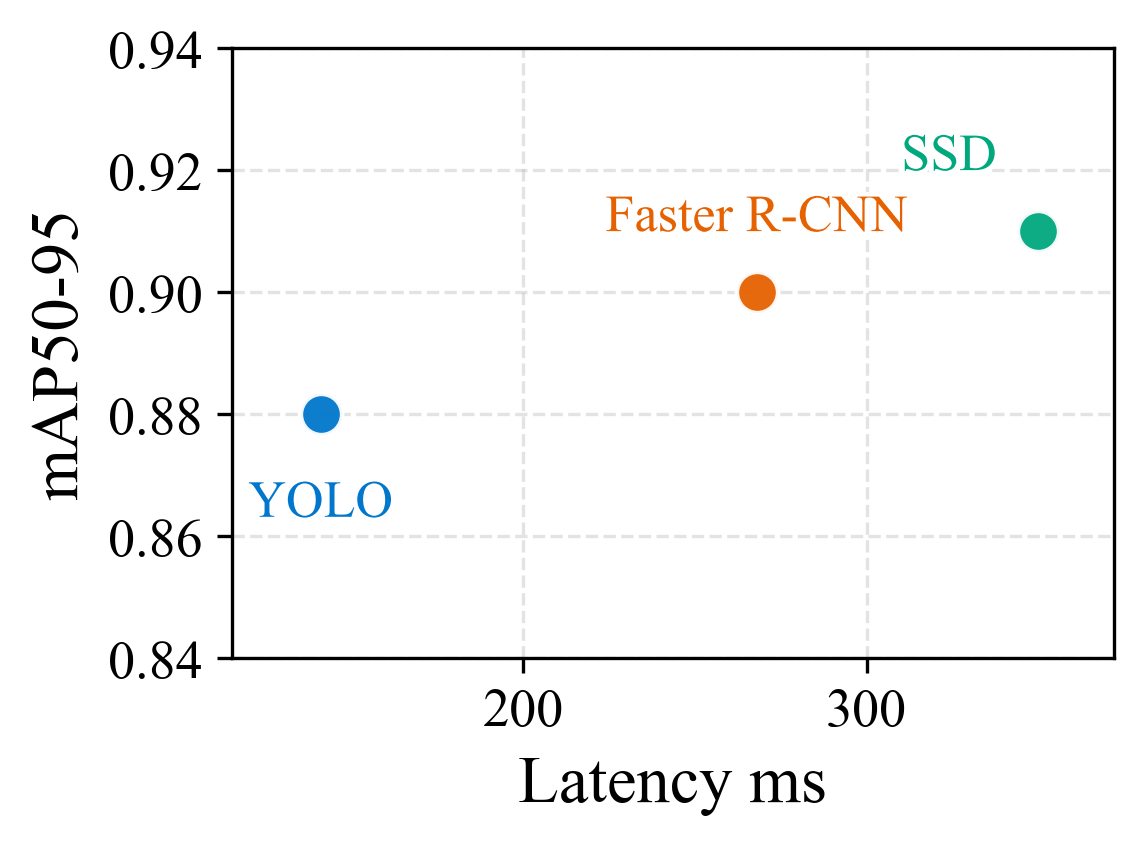
\includegraphics[width=\linewidth]{images/architecture_map_vs_latency_basic.png}
    \end{subfigure}
    \hfill
    \begin{subfigure}[t]{0.49\columnwidth}
        \caption{Datasets.}
        \label{fig:dataset_compare}
        \centering
        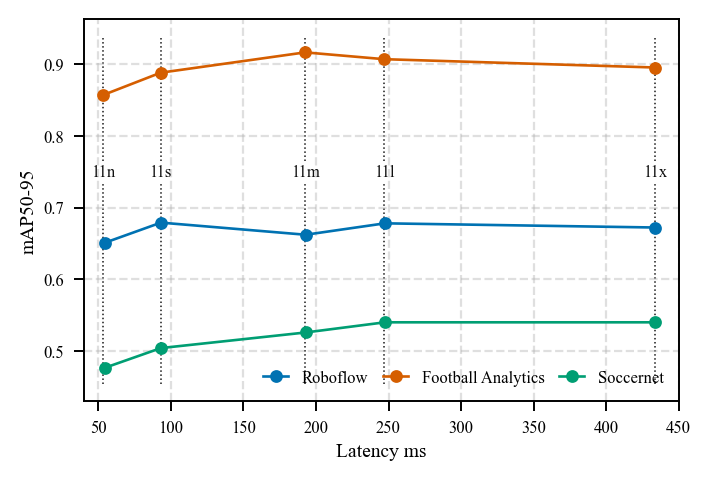
\includegraphics[width=\linewidth]{images/map50_95_vs_latency_11_non_ds3_ds3_soccernet.png}
    \end{subfigure}
\end{figure}

As can be seen from Figure \ref{fig:arch_compare}, although Faster R-CNN \cite{Zhao2023RTDETR} and SSD achieved slightly higher initial accuracy, the YOLO family \cite{UltralyticsYOLO} provided substantially lower latency on the Jetson Orin Nano Dev Kit. As a result, YOLO-based models were selected for the subsequent object detection experiments, as they offered the most suitable balance between accuracy and real-time edge deployment performance. Figure~\ref{fig:dataset_compare} indicates that the Football Analytics dataset achieved the strongest initial $\mathrm{mAP}_{50\text{--}95}$, at approximately 91\%, and was therefore selected for the majority of the object detection study.



\subsection{Summary of Model Training}



With the model family and dataset selected, the full training and compression study was then carried out. In total, 488 unique model artefacts were generated and evaluated across the object detection and pitch keypoint tasks. This included 104 \textbf{YOLO11} models, 152 \textbf{YOLO11-pose} models, 72 \textbf{YOLO26} models, and 160 \textbf{YOLO26-pose} models. The majority of the model inventory consisted of compressed variants rather than baseline models, reflecting the central aim of the study: to examine how different deployment-focused compression strategies affect performance on edge hardware. 

\subsection{Compression Analysis Summary}
Before individually exploring each compression technique and desired hardware resource reduction, it is useful to first summarise the overall trends across the full model inventory. The following tables and accompanying trade-off plots provide a high-level overview of how each compression technique and combination affected the mAP$_{50\text{--}95}$ versus latency relationship for the object detection and pitch keypoint models. These summaries allow the general patterns to be identified before delving into the more detailed per-technique analyses that follow.

\subsubsection{Compression Summaries: Object Models}
Table \ref{tab:object_technique_summary} below displays the average change in mAP50-95 and latency for each of the main optimisation techniques applied to the YOLO11 and YOLO26 object detection models, averaged across the paired N, S, M, L, and X variants.

\setcellcolorrange{0}{60}{70}
\begin{table}[H]
\centering
\caption{Object base optimisation summary.}
\label{tab:object_technique_summary}
\footnotesize
\definecolor{rulegray}{gray}{0.88}
\begin{minipage}{0.35\linewidth}
\centering
\setlength{\tabcolsep}{4pt}
\begin{tabular}{l c c}
\toprule
\textbf{Technique} & \textbf{$\Delta$mAP} & \textbf{Lat.$\downarrow$} \\
\midrule
\textbf{Acceleration} & \autocolorcell{-0.3}{-0.3\%} & \autocolorcell{31.0}{31.0\%} \\

\arrayrulecolor{rulegray}\specialrule{0.35pt}{0pt}{0pt}\arrayrulecolor{black}

\multicolumn{3}{l}{\textbf{Input Scaling and Accel.}} \\
\hspace{1em}75\% & \autocolorcell{-3.1}{-3.1\%} & \autocolorcell{31.5}{31.5\%} \\
\hspace{1em}60\% & \autocolorcell{-9.1}{-9.1\%} & \autocolorcell{52.9}{52.9\%} \\
\hspace{1em}50\% & \autocolorcell{-15.4}{-15.4\%} & \autocolorcell{67.7}{67.7\%} \\

\arrayrulecolor{rulegray}\specialrule{0.35pt}{0pt}{0pt}\arrayrulecolor{black}

\multicolumn{3}{l}{\textbf{Quantisation}} \\
\hspace{1em}FP16 & \autocolorcell{-1.6}{-1.6\%} & \autocolorcell{42.8}{42.8\%} \\
\hspace{1em}INT8 & \autocolorcell{-9.9}{-9.9\%} & \autocolorcell{52.6}{52.6\%} \\

\arrayrulecolor{rulegray}\specialrule{0.35pt}{0pt}{0pt}\arrayrulecolor{black}

\multicolumn{3}{l}{\textbf{Pruning}} \\
\hspace{1em}90\% pruning & \autocolorcell{-1.6}{-1.6\%} & \autocolorcell{2.3}{2.3\%} \\
\hspace{1em}80\% pruning & \autocolorcell{-2.4}{-2.4\%} & \autocolorcell{2.8}{2.8\%} \\
\hspace{1em}70\% pruning & \autocolorcell{-4.6}{-4.6\%} & \autocolorcell{13.4}{13.4\%} \\

\arrayrulecolor{rulegray}\specialrule{0.35pt}{0pt}{0pt}\arrayrulecolor{black}

\multicolumn{3}{l}{\textbf{Distillation}} \\
\hspace{1em}Small jump & \autocolorcell{-1.1}{-1.1\%} & \autocolorcell{-13.3}{-13.3\%} \\
\hspace{1em}Medium jump & \autocolorcell{-0.7}{-0.7\%} & \autocolorcell{-10.7}{-10.7\%} \\
\hspace{1em}Large jump & \autocolorcell{-2.1}{-2.1\%} & \autocolorcell{-8.7}{-8.7\%} \\
\bottomrule
\end{tabular}
\end{minipage}
\hfill
\begin{minipage}{0.64\linewidth}
\centering
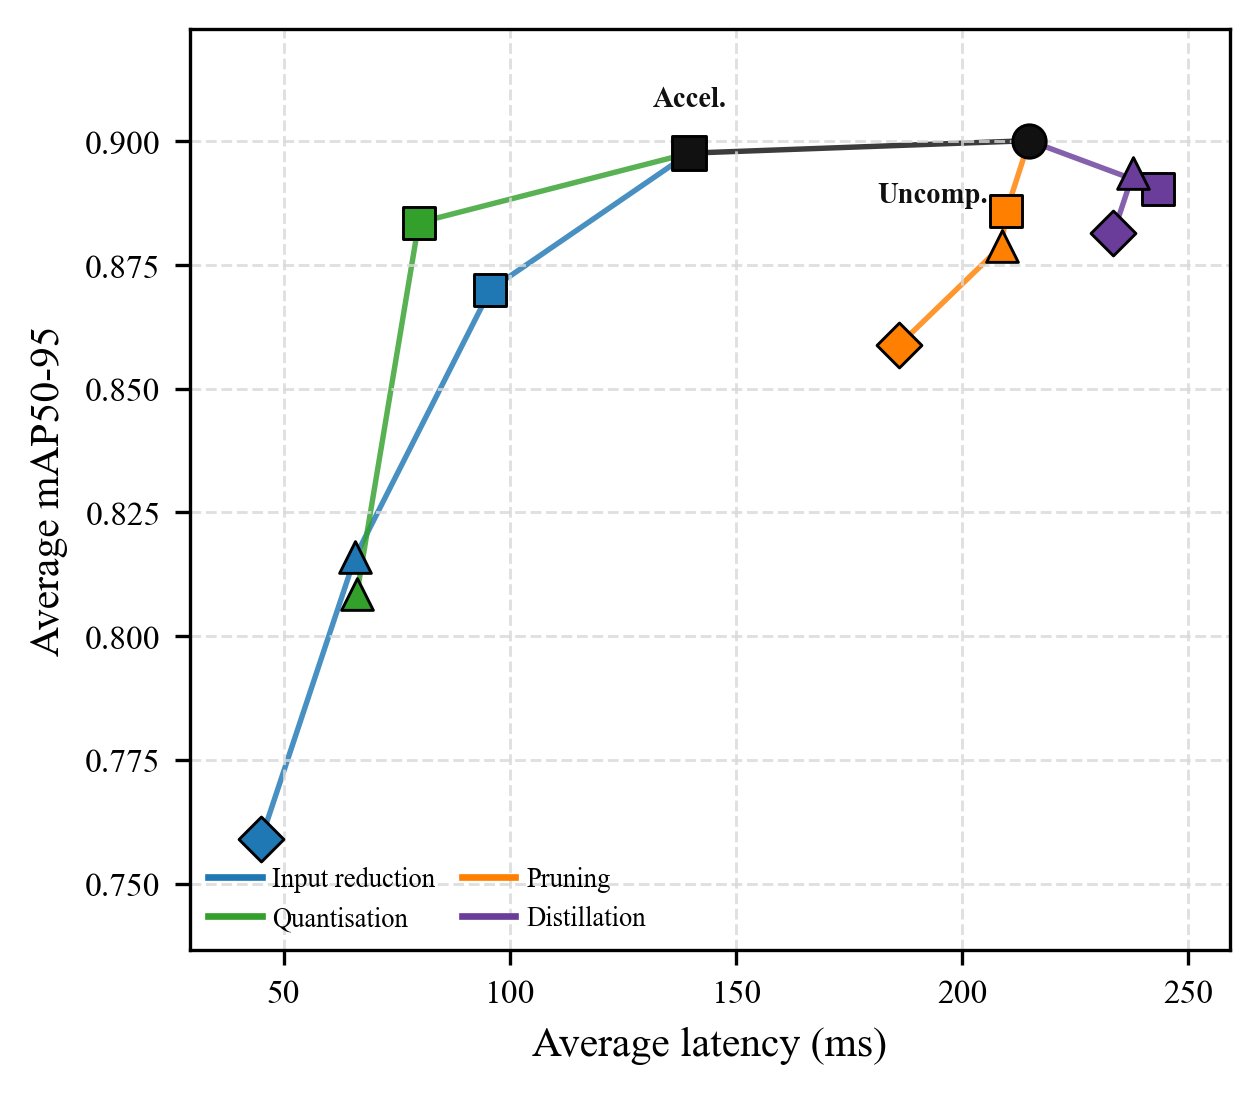
\includegraphics[width=\linewidth]{../Figures/produced_images/object_technique_summary_tradeoff.png}
\end{minipage}

\par
\vspace{3pt}
\noindent\parbox{\linewidth}{\footnotesize \textit{Note:} Distill Jump sizes defined by gap to teacher: small=1 size up, medium=2 sizes, large=3+ sizes up.}
\end{table}


Hardware acceleration can immediately be seen to be the most effective technique, reducing latency by \textbf{31.0\%} with only a \textbf{-0.3\%} change in mAP$_{50\text{--}95}$. FP16 quantisation also offers a significant latency improvement with little accuracy loss, delivering a \textbf{42.8\%} latency improvement for only a \textbf{-1.6\%} mAP$_{50\text{--}95}$ reduction. INT8 pushes latency lower at a clearer analytical cost. Input reduction then becomes a more incremental trade-off: $960\times960$ px gives a similar latency gain to acceleration, with a larger analytical penalty, while $768\times768$ px and $640\times640$ px produce a much steeper trade-off. In the checkpoint-level \texttt{.pt} comparison, pruning provides only a small average runtime gain until the most aggressive setting, while distillation actually moves latency in the wrong direction on average despite keeping the mAP$_{50\text{--}95}$ loss relatively small. This reinforces the idea that knowledge distillation is more useful as a training intervention than as a direct compression strategy. The combination of these various techniques can now be explored, as shown in Table \ref{tab:object_combo_summary}. 


\setcellcolorrange{0}{60}{70}
\begin{table}[H]
\footnotesize
\centering
\caption{Object combined compression summary.}
\label{tab:object_combo_summary}
\definecolor{rulegray}{gray}{0.88}
\begin{minipage}{0.3\linewidth}
\centering
\setlength{\tabcolsep}{4pt}
\begin{tabular}{l c c}
\toprule
\textbf{Combination} & \textbf{$\Delta$mAP} & \textbf{Lat. $\downarrow$} \\
\midrule
\multicolumn{3}{l}{\textbf{Distilled And}} \\
\hspace{1em}Accelerated & \autocolorcell{-1.5}{-1.5\%} & \autocolorcell{23.4}{23.4\%} \\
\hspace{1em}FP16 & \autocolorcell{-2.8}{-2.8\%} & \autocolorcell{42.0}{42.0\%} \\
\hspace{1em}INT8 & \autocolorcell{-8.9}{-8.9\%} & \autocolorcell{42.9}{42.9\%} \\

\arrayrulecolor{rulegray}\specialrule{0.35pt}{0pt}{0pt}\arrayrulecolor{black}

\multicolumn{3}{l}{\textbf{Pruned And}} \\
\hspace{1em}Accelerated & \autocolorcell{-2.8}{-2.8\%} & \autocolorcell{40.5}{40.5\%} \\
\hspace{1em}FP16 & \autocolorcell{-4.4}{-4.4\%} & \autocolorcell{61.6}{61.6\%} \\
\hspace{1em}INT8 & \autocolorcell{-10.1}{-10.1\%} & \autocolorcell{65.6}{65.6\%} \\

\arrayrulecolor{rulegray}\specialrule{0.35pt}{0pt}{0pt}\arrayrulecolor{black}

\multicolumn{3}{l}{\textbf{Distill+Prune And}} \\
\hspace{1em}Accelerated & \autocolorcell{-2.2}{-2.2\%} & \autocolorcell{23.1}{23.1\%} \\
\hspace{1em}FP16 & \autocolorcell{-3.3}{-3.3\%} & \autocolorcell{37.7}{37.7\%} \\
\hspace{1em}INT8 & \autocolorcell{-8.6}{-8.6\%} & \autocolorcell{37.3}{37.3\%} \\
\bottomrule
\end{tabular}
\end{minipage}
\hfill
\begin{minipage}{0.65\linewidth}
\centering
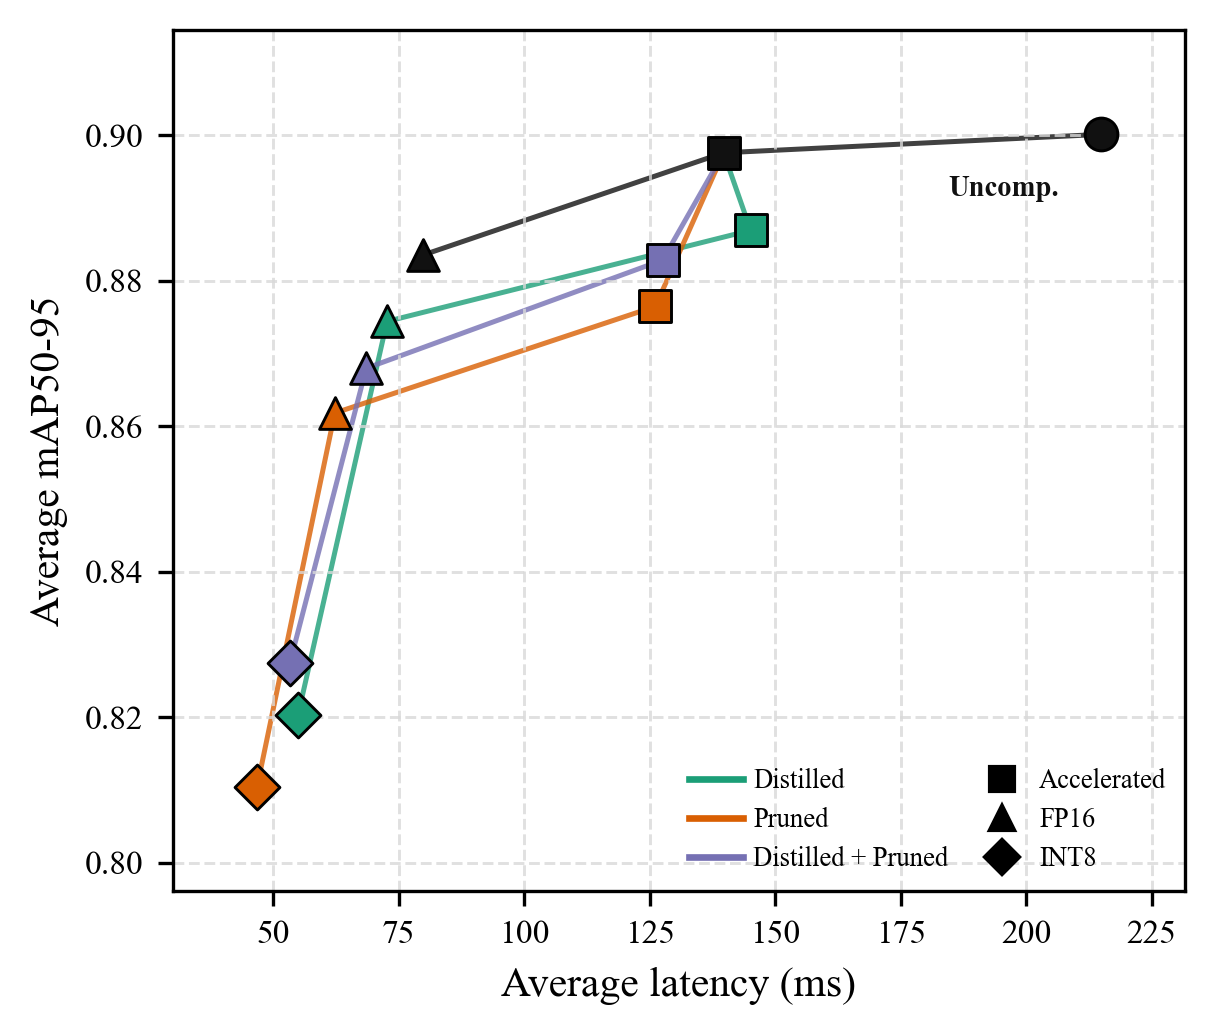
\includegraphics[width=\linewidth]{../Figures/produced_images/object_combo_summary_tradeoff.png}
\end{minipage}
\end{table}


As can be seen in Table \ref{tab:object_combo_summary}, there is essentially no downside to hardware acceleration. By contrast, distillation, pruning, and a combination of the two introducw trade-offs, with increases in latency and reductions in mAP$_{50\text{--}95}$ that become more pronounced as the compression path becomes more aggressive. The most extreme combined paths, which include INT8 quantisation, achieve the largest latency improvements but also the largest mAP$_{50\text{--}95}$ reductions. The FP16-based combined paths occupy a more balanced middle ground, providing substantial latency improvements while preserving much more of the analytical performance than the INT8 routes. Overall, these summary tables indicate that hardware acceleration is a clear first step for improving deployability, while more aggressive compression techniques require careful consideration of the accuracy--latency trade-off. 


With a summary of the object detection compression results, the optimisation of pitch keypoint models can now be examined in the same way.
\subsubsection{Keypoint Detection Model Compression Summary}
\noindent Figure \ref{tab:pose_technique_summary} display the same summary view to thepitch keypoint models produced, averaging the effect of each base technique across the paired N, S, M, L, and X variants.

\setcellcolorrange{0}{60}{70}
\begin{table}[H]
\centering
\caption{Pose base optimisation summary.}
\label{tab:pose_technique_summary}
\footnotesize
\definecolor{rulegray}{gray}{0.88}
\begin{minipage}{0.35\linewidth}
\centering
\setlength{\tabcolsep}{4pt}
\begin{tabular}{l c c}
\toprule
\textbf{Technique} & \textbf{$\Delta$mAP} & \textbf{Lat.$\downarrow$} \\
\midrule
\textbf{Acceleration} & \autocolorcell{0.0}{0.0\%} & \autocolorcell{35.5}{35.5\%} \\

\arrayrulecolor{rulegray}\specialrule{0.35pt}{0pt}{0pt}\arrayrulecolor{black}

\multicolumn{3}{l}{\textbf{Input Scaling and Accel.}} \\
\hspace{1em}960 & \autocolorcell{-18.2}{-18.2\%} & \autocolorcell{12.5}{12.5\%} \\
\hspace{1em}768 & \autocolorcell{-28.2}{-28.2\%} & \autocolorcell{45.0}{45.0\%} \\
\hspace{1em}640 & \autocolorcell{-47.6}{-47.6\%} & \autocolorcell{62.8}{62.8\%} \\

\arrayrulecolor{rulegray}\specialrule{0.35pt}{0pt}{0pt}\arrayrulecolor{black}

\multicolumn{3}{l}{\textbf{Quantisation}} \\
\hspace{1em}FP16 & \autocolorcell{0.1}{0.1\%} & \autocolorcell{43.1}{43.1\%} \\
\hspace{1em}INT8 & \autocolorcell{-43.8}{-43.8\%} & \autocolorcell{53.0}{53.0\%} \\

\arrayrulecolor{rulegray}\specialrule{0.35pt}{0pt}{0pt}\arrayrulecolor{black}

\multicolumn{3}{l}{\textbf{Pruning}} \\
\hspace{1em}90\% pruning & \autocolorcell{-24.5}{-24.5\%} & \autocolorcell{3.9}{3.9\%} \\
\hspace{1em}80\% pruning & \autocolorcell{-23.6}{-23.6\%} & \autocolorcell{3.2}{3.2\%} \\
\hspace{1em}70\% pruning & \autocolorcell{-26.2}{-26.2\%} & \autocolorcell{4.7}{4.7\%} \\

\arrayrulecolor{rulegray}\specialrule{0.35pt}{0pt}{0pt}\arrayrulecolor{black}

\multicolumn{3}{l}{\textbf{Distillation}} \\
\hspace{1em}Small jump & \autocolorcell{-2.2}{-2.2\%} & \autocolorcell{-6.8}{-6.8\%} \\
\hspace{1em}Medium jump & \autocolorcell{-3.2}{-3.2\%} & \autocolorcell{-5.1}{-5.1\%} \\
\hspace{1em}Large jump & \autocolorcell{-1.9}{-1.9\%} & \autocolorcell{-4.3}{-4.3\%} \\
\bottomrule
\end{tabular}
\end{minipage}
\hfill
\begin{minipage}{0.64\linewidth}
\centering
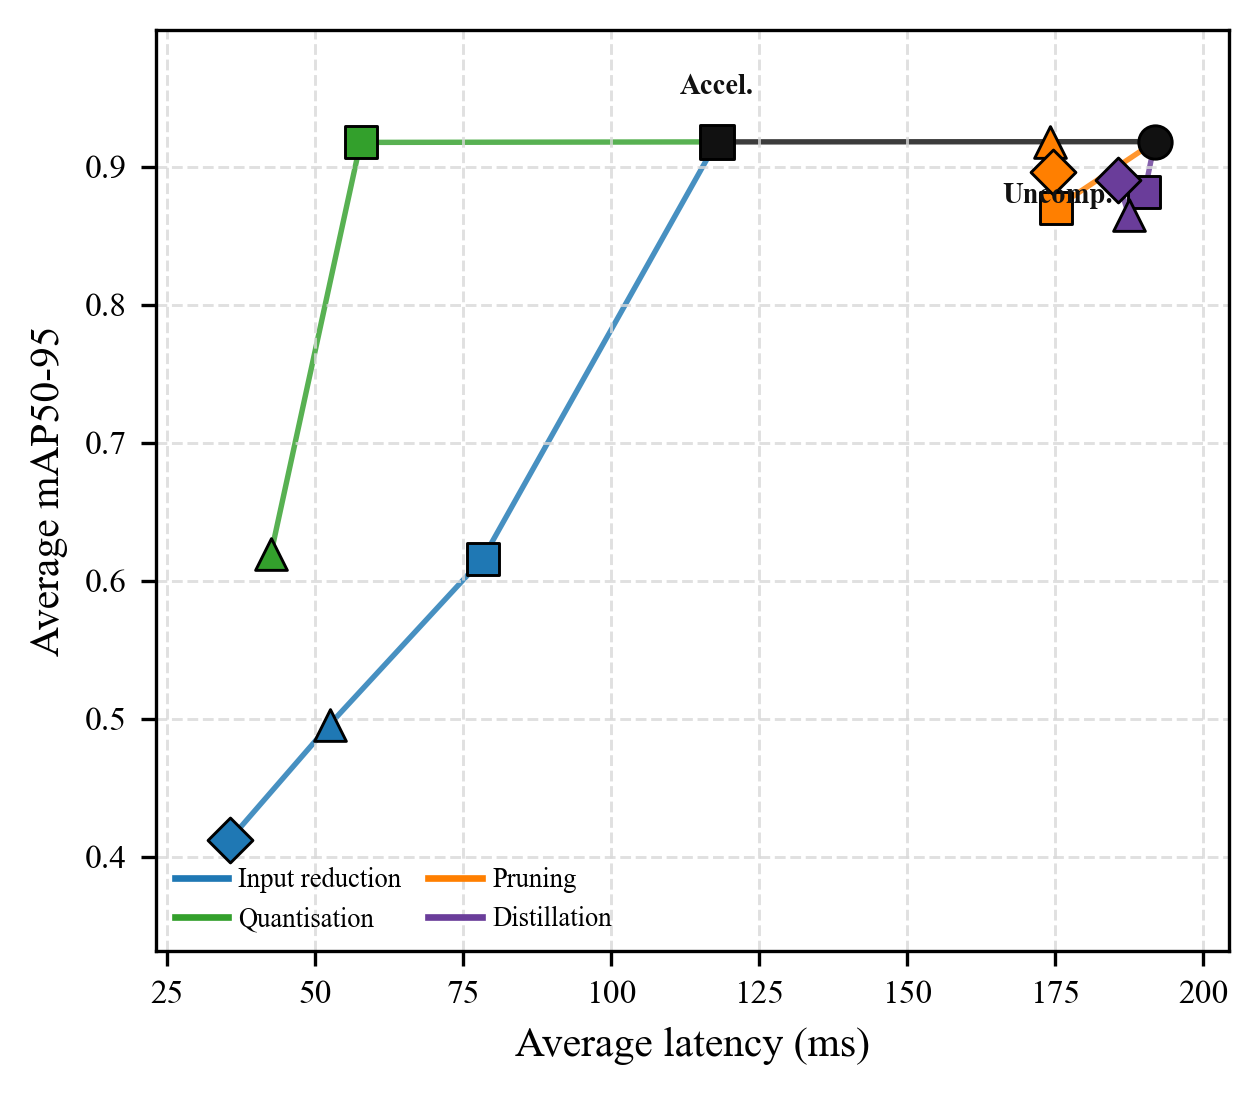
\includegraphics[width=\linewidth]{../Figures/produced_images/pose_technique_summary_tradeoff.png}
\end{minipage}

\par
\vspace{3pt}
\noindent\parbox{\linewidth}{\footnotesize \textit{Note:} Distill Jump sizes defined by gap to teacher: small=1 size up, medium=2 sizes, large=3+ sizes up.}
\end{table}


Figure \ref{tab:pose_technique_summary} shows that the same techniques that were effective for object detection also produce the strongest latency improvements for keypoint estimation, with hardware acceleration and quantisation again leading the way. However, the mAP$_{50\text{--}95}$ reductions are generally more severe for the pose models than for the object models, especially for input resolution reduction and pruning. This indicates that the keypoint task is more sensitive to aggressive compression. 

 Table \ref{tab:pose_combo_summary} and its companion trade-off plot extend this comparison to the YOLO26-pose combined compression paths.

\setcellcolorrange{0}{60}{70}
\begin{figure}[H]
\footnotesize
\centering
\caption{Keypoint Model Combined Compression Summary.}
\label{fig:pose_combo_summary}
\definecolor{rulegray}{gray}{0.88}
\definecolor{colorpruned}{HTML}{d95f02}
\definecolor{colordistillpruned}{HTML}{7570b3}
\definecolor{colordistilled}{HTML}{33a02c}
\definecolor{colorquantized}{HTML}{1f78b4}
\begin{minipage}{0.33\linewidth}
\centering
\setlength{\tabcolsep}{3pt}
\resizebox{\linewidth}{!}{%
\begin{tabular}{l c c}
\toprule
\textbf{Combination} & \textbf{$\Delta$mAP} & \textbf{Lat. $\downarrow$} \\
\midrule
\multicolumn{3}{l}{\textbf{Pruned And}~\textcolor{colorpruned}{\rule[0.5ex]{1.3em}{2.5pt}}} \\
\hspace{1em}\textcolor{colorpruned}{$\blacksquare$}~Accelerated & \autocolorcell{-6.2}{-6.2\%} & \autocolorcell{9.0}{9.0\%} \\
\hspace{1em}\textcolor{colorpruned}{$\blacktriangle$}~960 & \autocolorcell{-6.5}{-6.5\%} & \autocolorcell{37.5}{37.5\%} \\
\hspace{1em}\textcolor{colorpruned}{\scalebox{1.2}[1]{$\blacklozenge$}}~FP16 & \autocolorcell{-6.2}{-6.2\%} & \autocolorcell{52.2}{52.2\%} \\
\hspace{1em}\textcolor{colorpruned}{$\bigstar$}~960+FP16 & \autocolorcell{-6.4}{-6.4\%} & \autocolorcell{58.8}{58.8\%} \\
\hspace{1em}\textcolor{colorpruned}{$\blacktriangledown$}~INT8 & \autocolorcell{-11.8}{-11.8\%} & \autocolorcell{59.2}{59.2\%} \\

\arrayrulecolor{rulegray}\specialrule{0.35pt}{0pt}{0pt}\arrayrulecolor{black}

\multicolumn{3}{l}{\textbf{Distill+Prune And}~\textcolor{colordistillpruned}{\rule[0.5ex]{1.3em}{2.5pt}}} \\
\hspace{1em}\textcolor{colordistillpruned}{$\blacksquare$}~Accelerated & \autocolorcell{-0.2}{-0.2\%} & \autocolorcell{44.2}{44.2\%} \\
\hspace{1em}\textcolor{colordistillpruned}{\scalebox{1.2}[1]{\scalebox{1.2}[1]{$\blacklozenge$}}}~FP16 & \autocolorcell{-0.3}{-0.3\%} & \autocolorcell{56.4}{56.4\%} \\

\arrayrulecolor{rulegray}\specialrule{0.35pt}{0pt}{0pt}\arrayrulecolor{black}

\multicolumn{3}{l}{\textbf{Distilled And}~\textcolor{colordistilled}{\rule[0.5ex]{1.3em}{2.5pt}}} \\
\hspace{1em}\textcolor{colordistilled}{$\blacksquare$}~Accelerated & \autocolorcell{0.9}{+0.9\%} & \autocolorcell{36.3}{36.3\%} \\
\hspace{1em}\textcolor{colordistilled}{$\blacktriangle$}~960 & \autocolorcell{3.3}{+3.3\%} & \autocolorcell{57.8}{57.8\%} \\
\hspace{1em}\textcolor{colordistilled}{\scalebox{1.2}[1]{$\blacklozenge$}}~FP16 & \autocolorcell{1.0}{+1.0\%} & \autocolorcell{68.7}{68.7\%} \\

\arrayrulecolor{rulegray}\specialrule{0.35pt}{0pt}{0pt}\arrayrulecolor{black}

\multicolumn{3}{l}{\textbf{FP16 And}~\textcolor{colorquantized}{\rule[0.5ex]{1.3em}{2.5pt}}} \\
\hspace{1em}\textcolor{colorquantized}{$\blacktriangle$}~960 & \autocolorcell{-33.1}{-33.1\%} & \autocolorcell{63.6}{63.6\%} \\
\hspace{1em}\textcolor{colorquantized}{$\blacktriangleright$}~768 & \autocolorcell{-46.0}{-46.0\%} & \autocolorcell{73.9}{73.9\%} \\
\hspace{1em}\textcolor{colorquantized}{$\blacktriangleleft$}~640 & \autocolorcell{-54.9}{-54.9\%} & \autocolorcell{82.8}{82.8\%} \\
\bottomrule
\end{tabular}
}
\end{minipage}
\hfill
\begin{minipage}{0.65\linewidth}
\centering
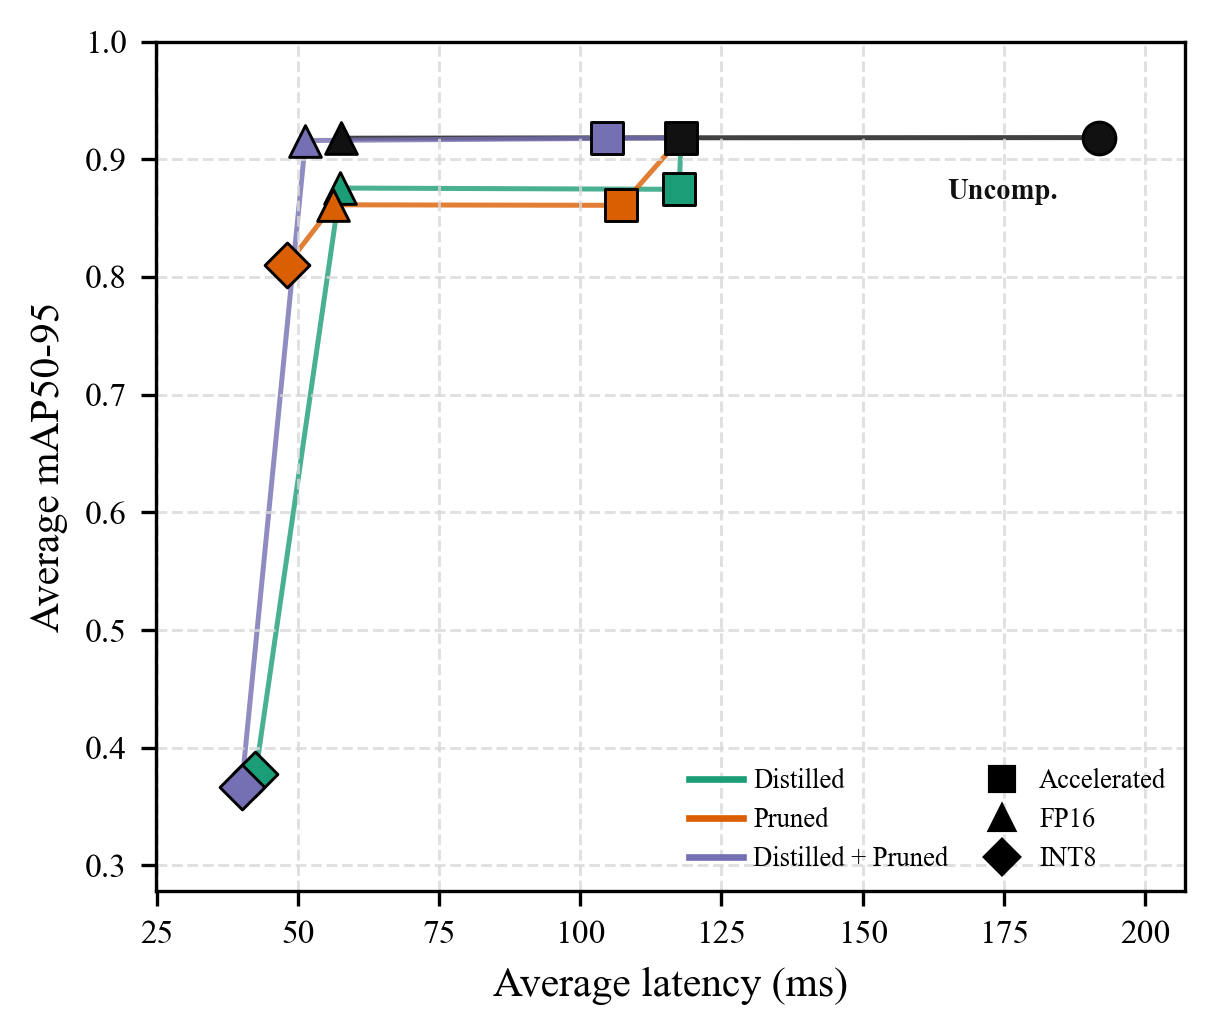
\includegraphics[width=\linewidth]{../Figures/produced_images/pose_combo_summary_tradeoff.png}
\end{minipage}
\end{figure}


The main takeaway of Figure \ref{tab:pose_combo_summary} is that INT8 quantisation is severely detrimental to performance. Beyond that

With a broad analysis of the effect of compression techniques on both object, and pose models, a more in-depth examination of each technique can now be carried out, exploring the effect of model size on compression efficiency.

\subsection{Compression Technique Analysis}

To explore each technique, a ploy of each individual model family is shown, demonstrating the mAP$_{50\text{--}95}$ versus latency trade-off as each technique is applied at various levels of compression aggression. First, hardware acceleration will be explored.

\subsubsection{Hardware Acceleration}
Figure \ref{fig:hardware_acceleration_results} presents the mAP50-95 versus latency relationship for the uncompressed and FP32-accelerated YOLO11 and YOLO26 object and pose model families. Rather than averaging the YOLO11 and YOLO26 variants at each model scale, the figure separates them into four panels so that the effect of TensorRT-based hardware acceleration can be compared directly across both architecture and task type. This makes it easier to see whether the same leftward latency shift is preserved for each family while retaining the scale-wise accuracy ordering within each panel.

\begin{figure}[H]
    \centering
    \caption{Hardware acceleration trade-off by architecture and task.}
    \label{fig:hardware_acceleration_results}
    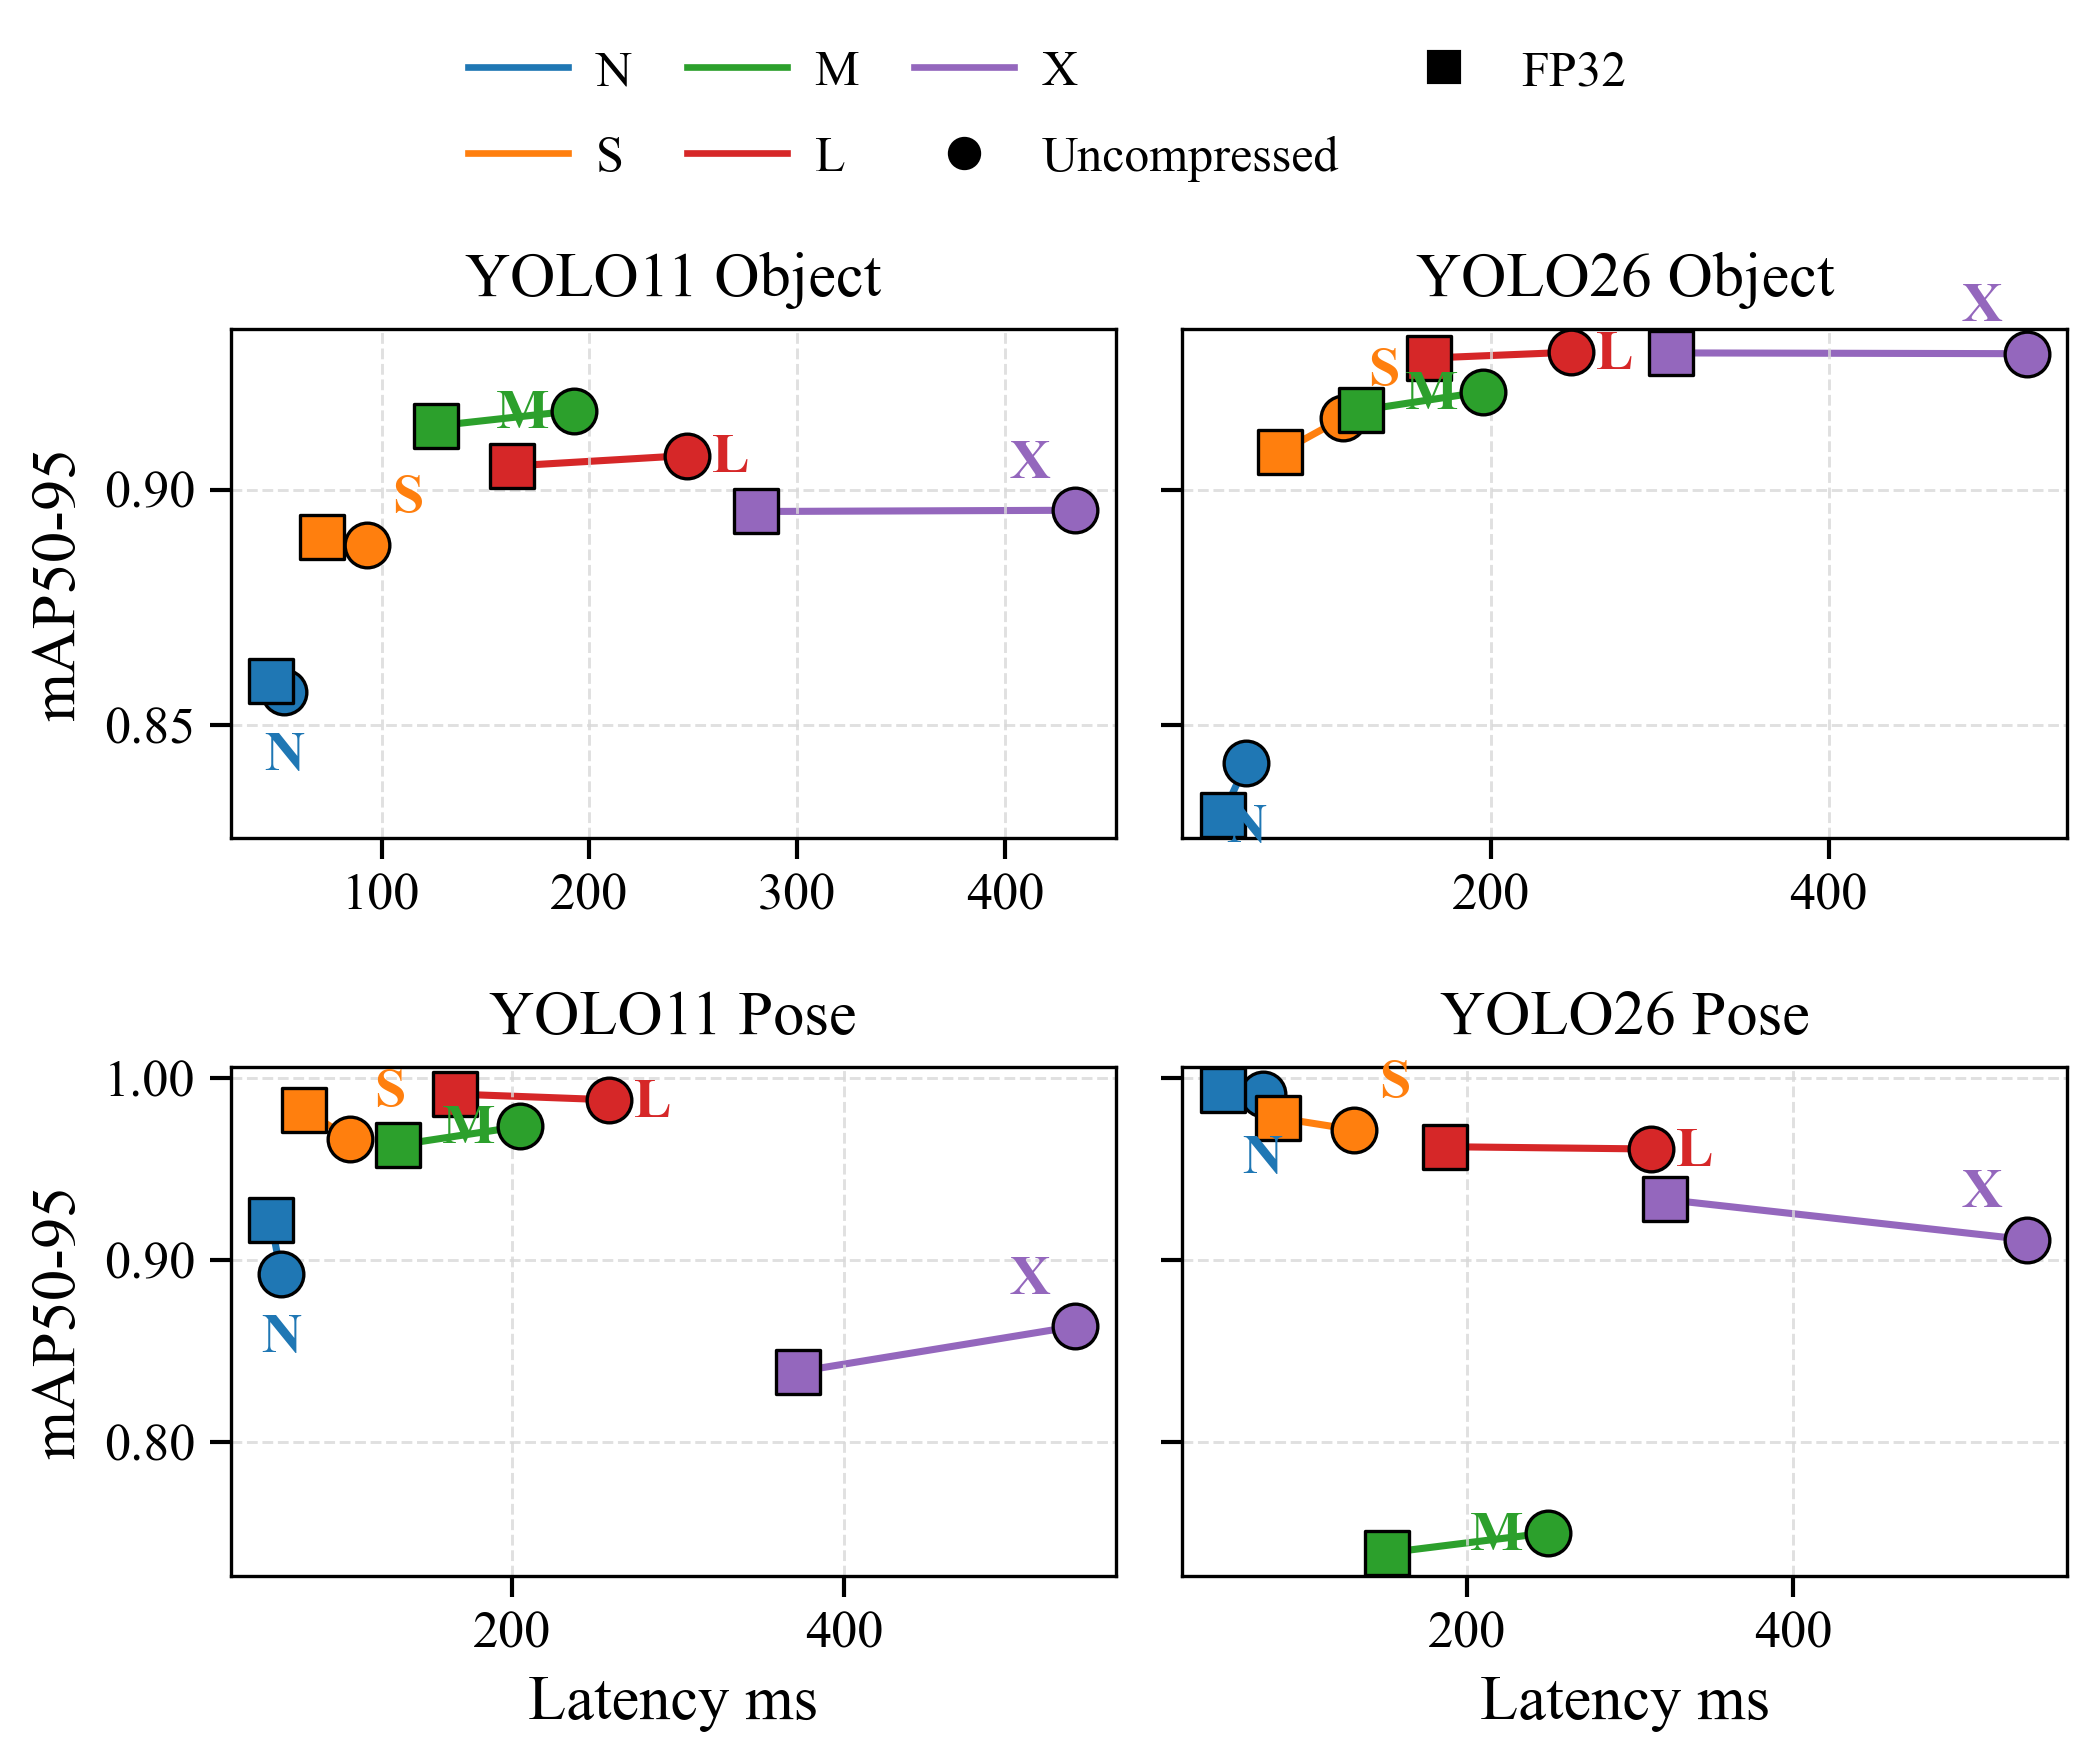
\includegraphics[width=\linewidth]{../Figures/produced_images/map50_95_vs_latency_baseline_pairs.png}
\end{figure}

The results show that hardware acceleration provides a substantial reduction in latency across all model scales while preserving almost identical mAP50-95 performance. In each family-task group, the FP32-accelerated points move consistently leftward relative to their uncompressed counterparts, indicating faster inference with negligible accuracy loss. This suggests that deployment optimisation alone provides a strong baseline improvement before more aggressive compression techniques are considered. It is also notable that the relative ordering of the models is preserved after acceleration, meaning that larger models remain more accurate but slower, while smaller models remain faster but less accurate. Overall, hardware acceleration improves deployability without materially altering the underlying accuracy hierarchy.


\subsubsection{Input Resolution Reduction}


Figure \ref{fig:input_resolution_reduction_results} shows the effect of reducing the input resolution on the mAP50-95 versus latency trade-off for the YOLO11 and YOLO26 object and pose models. Each line traces the progression of a family-task group through increasingly aggressive input resolution reduction, allowing the effect of this technique to be examined in a structured way across both model scale and task type.
\begin{figure}[H]
    \centering
    \caption{Input resolution reduction trade-off.}
    \label{fig:input_resolution_reduction_results}
    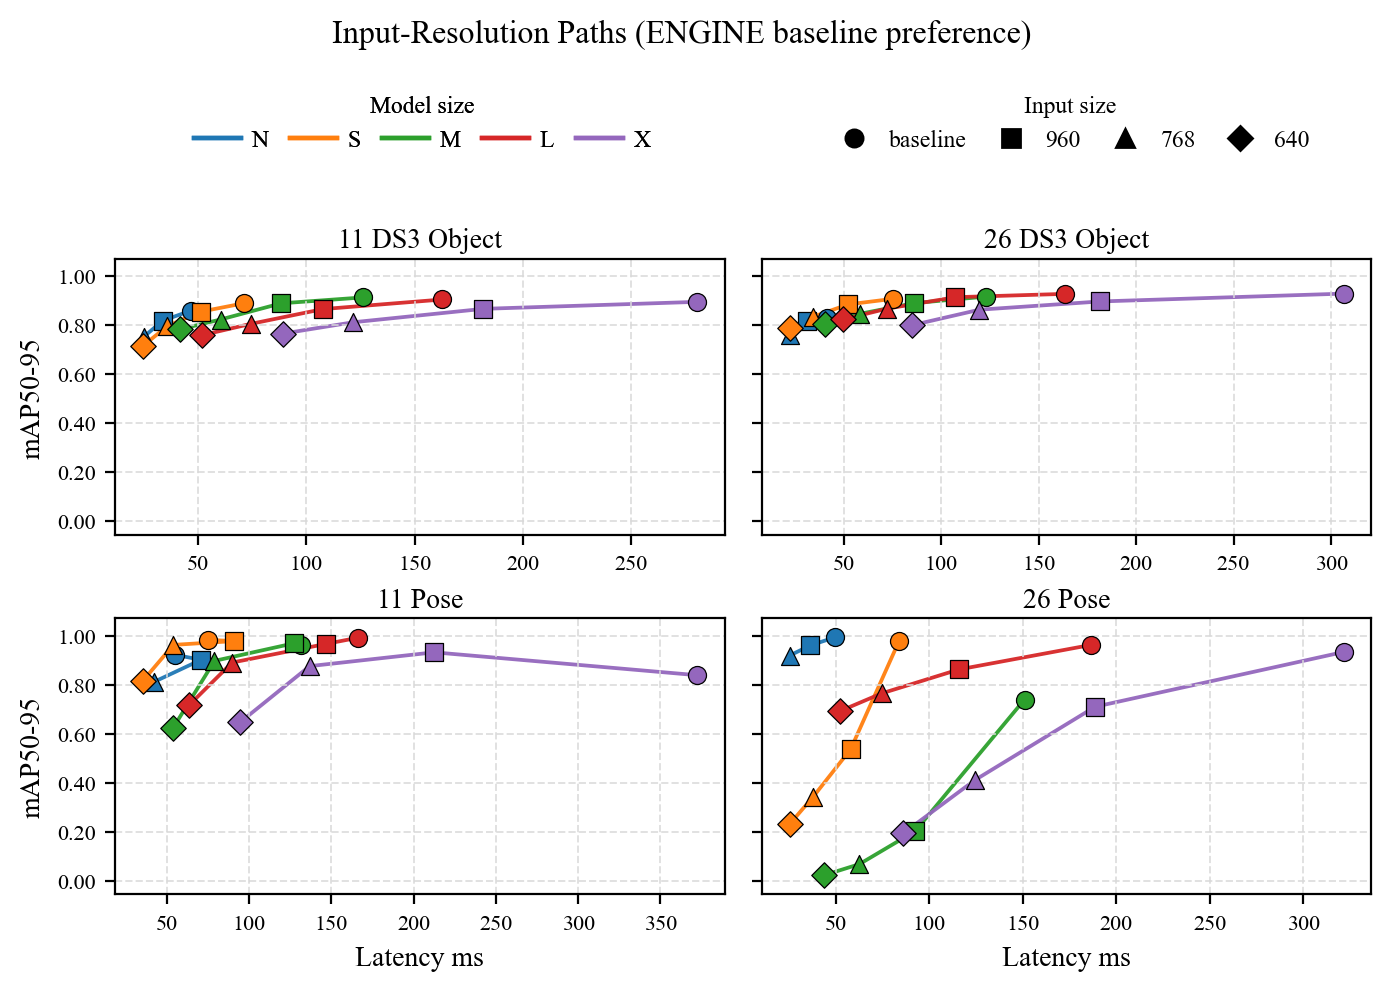
\includegraphics[width=\linewidth]{../Figures/produced_images/map50_95_vs_latency_input_resolution_panels.png}
\end{figure}

As shown in Figure \ref{fig:input_resolution_reduction_results}, reducing the input resolution produces a significant reduction in latency for all four model families. The object detection models preserve relatively high mAP50-95 values alongside this latency reduction. By contrast, the pose models, and especially the YOLO26 pose variants, experience substantially larger degradations in accuracy as resolution decreases. This indicates that input resolution reduction is considerably more tolerable for object detection than for keypoint estimation,. 


\subsubsection{Quantisation}
Figure \ref{fig:quantisation_results} shows the average mAP50-95 versus latency trade-off for baseline, FP32, and INT8 deployment stages across the YOLO11 and YOLO26 object and pose families. Each line traces the progression of a family-task group through increasingly aggressive deployment optimisation, allowing the effect of quantisation on both inference speed and accuracy retention to be examined in a structured way. This makes it possible to compare whether object and pose models respond similarly to reduced numerical precision.

\begin{figure}[H]
    \centering
    \caption{Quantisation trade-off.}
    \label{fig:quantisation_results}
    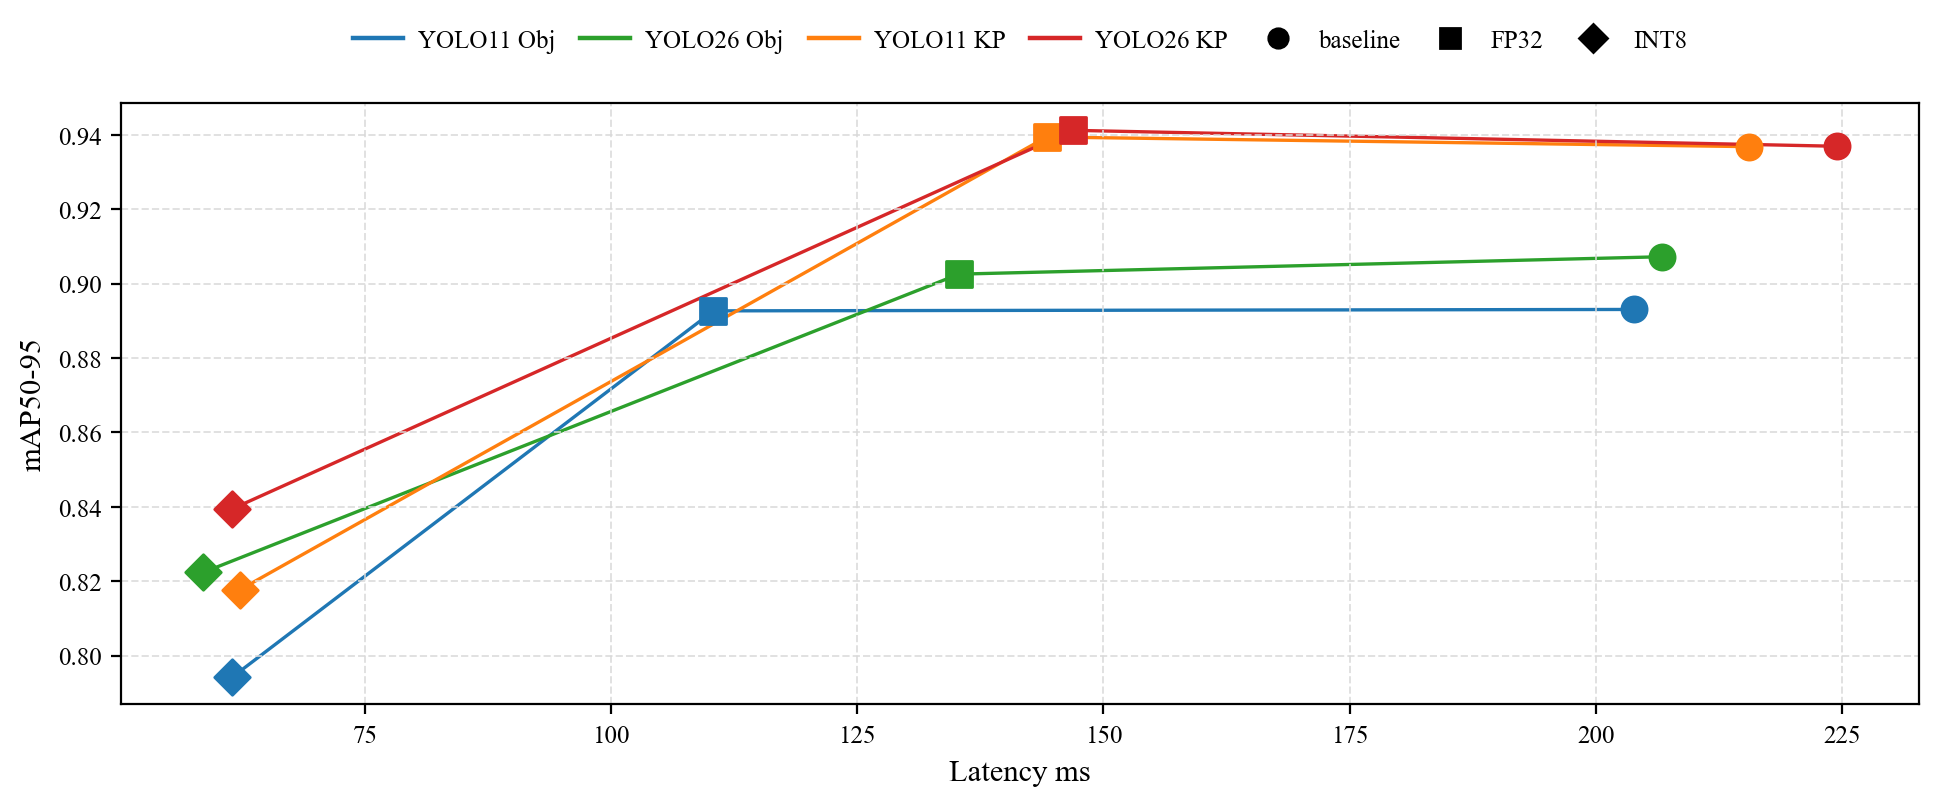
\includegraphics[width=\linewidth]{images/map50_95_vs_latency_quant_pairs.png}
\end{figure}

The figure shows that quantisation produces clear latency improvements, with INT8 giving the largest speedup in every family-task group. However, the associated accuracy cost is much more pronounced than in the hardware acceleration case. FP32 acceleration preserves accuracy almost exactly, whereas the move to INT8 shifts the points further left but also noticeably downward. This effect is particularly clear for the object models, where latency is reduced substantially but mAP50-95 falls by a visible margin. The pose models also experience a drop, though they remain at relatively high absolute accuracy. Overall, the results indicate that quantisation is effective for improving runtime efficiency, but that the gain is achieved through a more explicit accuracy--latency trade-off than hardware acceleration alone.

\subsubsection{Pruning}
Figure \ref{fig:pruning_results} illustrates the mAP50-95 versus latency relationship for YOLO11 object and pose models under increasing pruning strength. Separate N, S, M, and L lines are shown for the baseline, P90, P80, and P70 checkpoints, allowing the effect of structured pruning to be examined both across pruning intensity and across model scale. This presentation makes it possible to assess whether pruning shifts the models toward a more favourable operating point or instead introduces excessive accuracy degradation.

\begin{figure}[H]
    \centering
    \caption{Pruning trade-off.}
    \label{fig:pruning_results}
    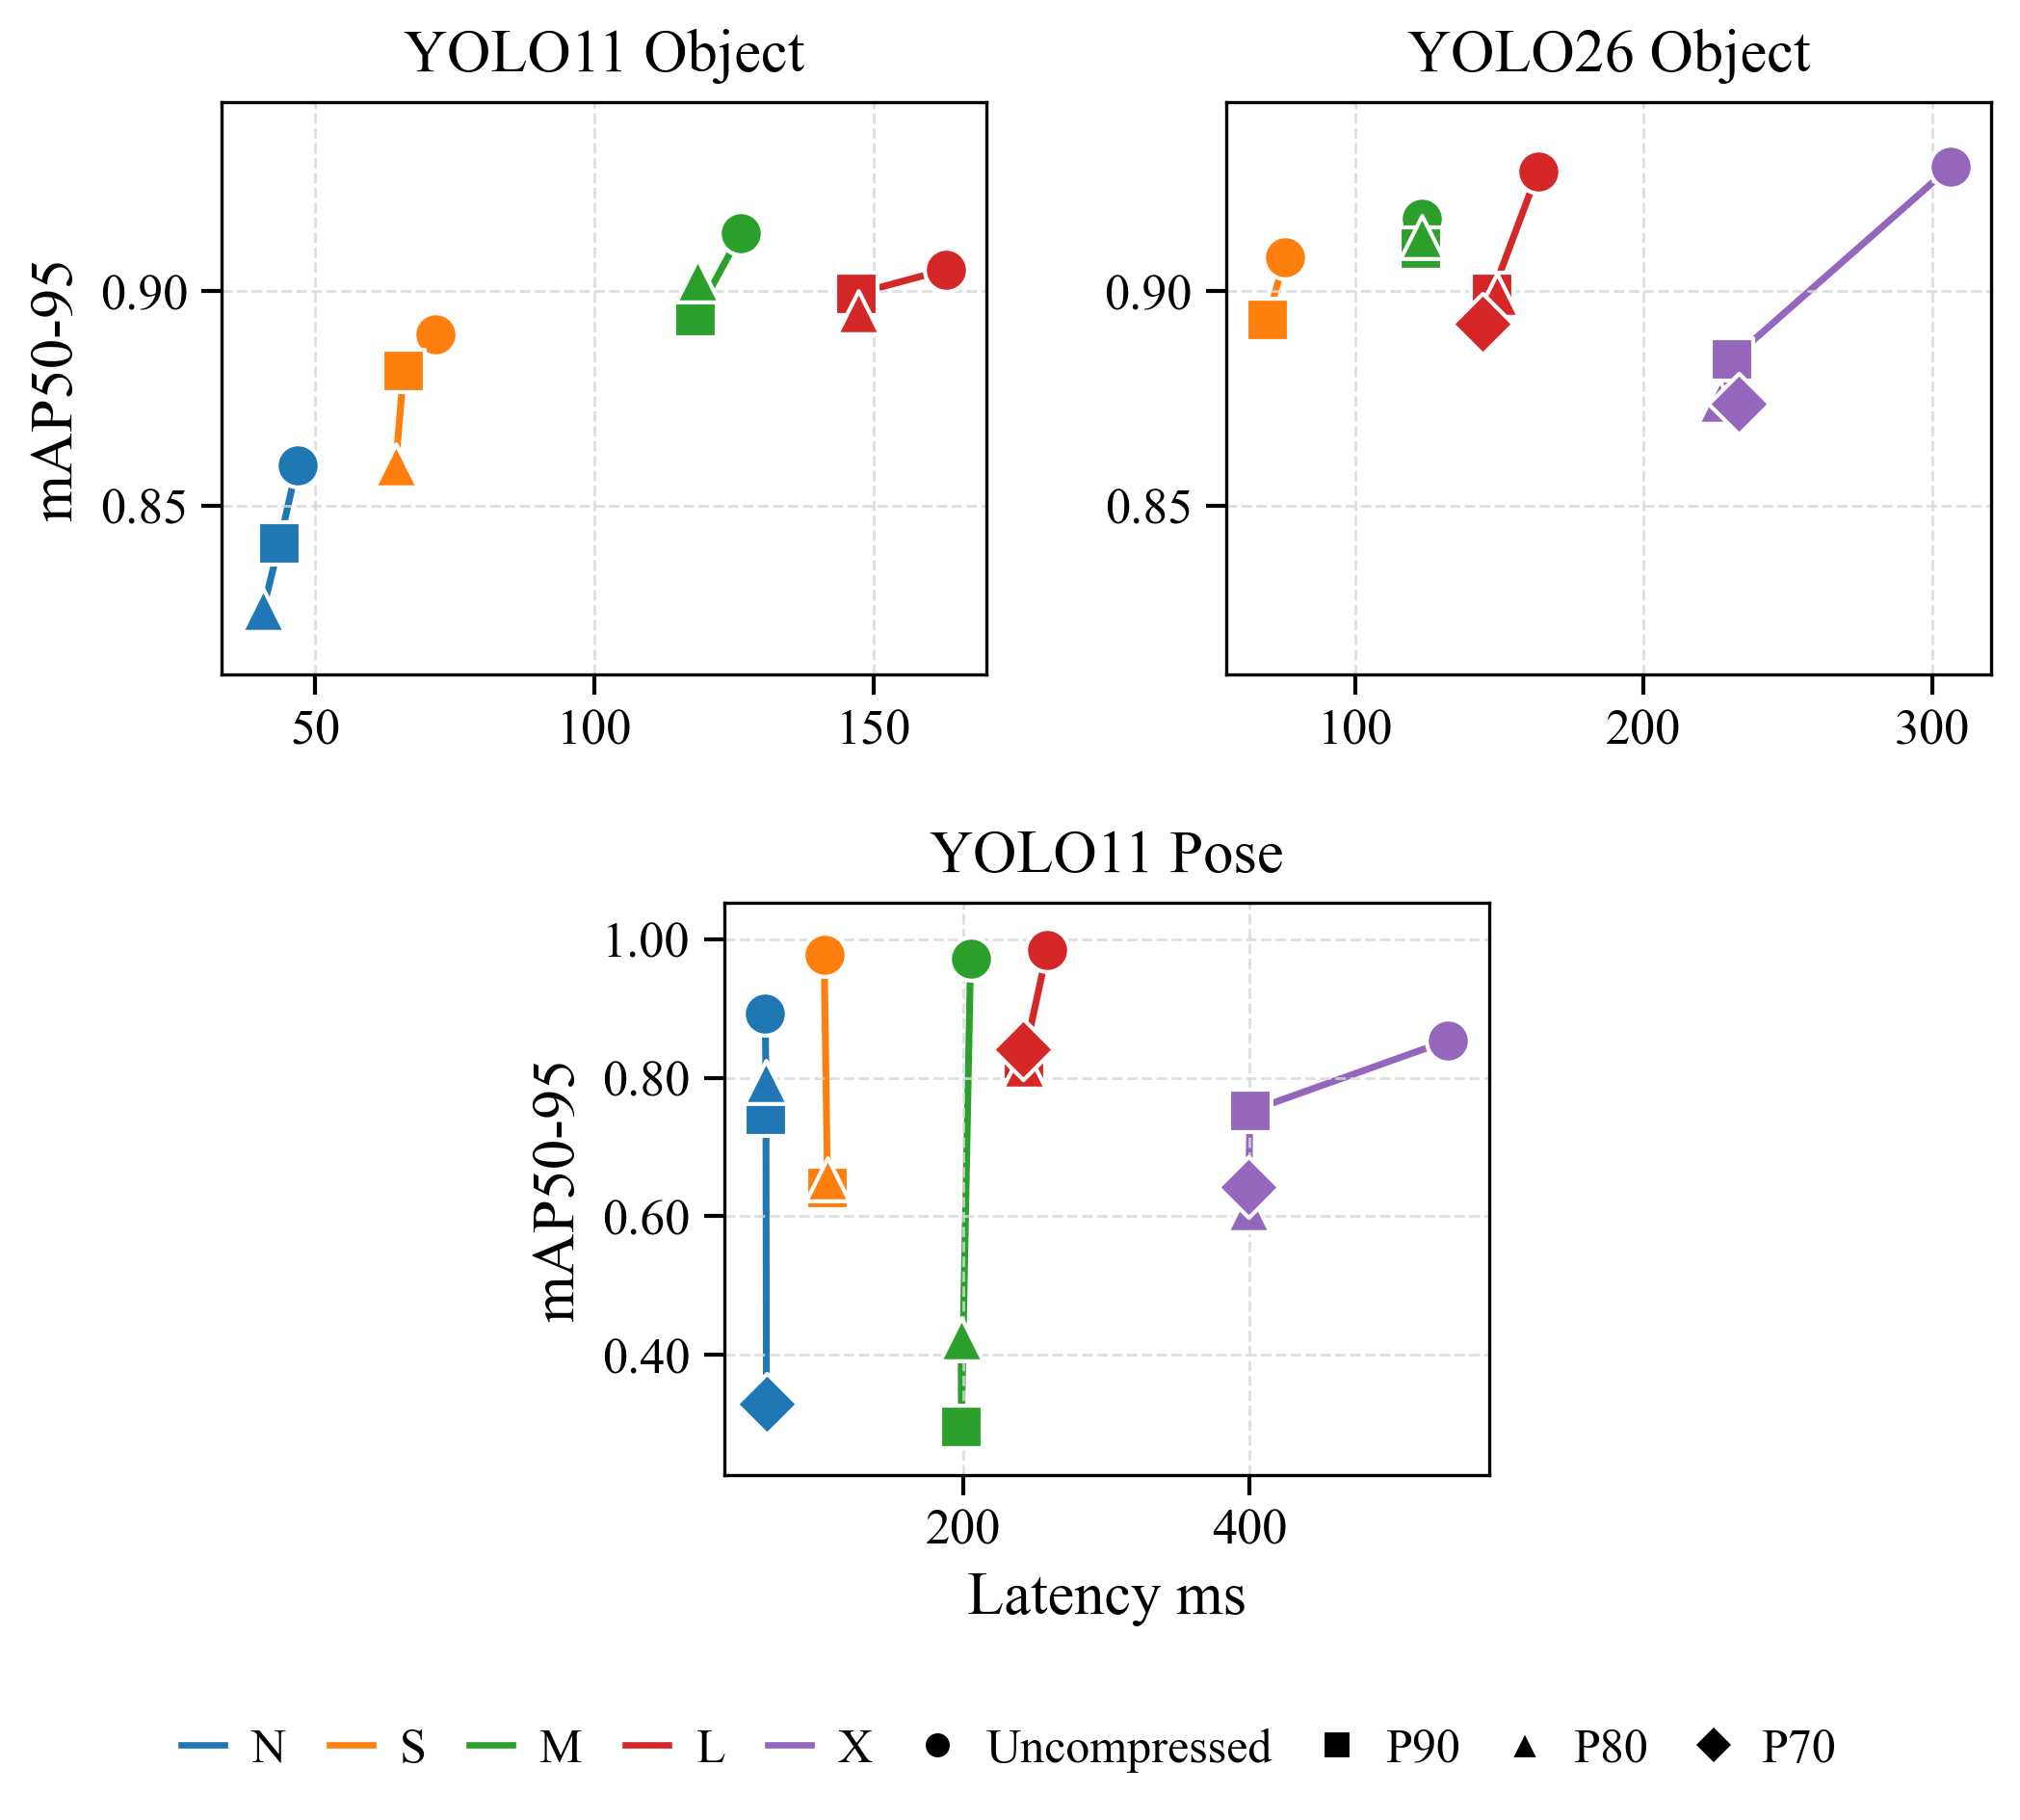
\includegraphics[width=\linewidth]{images/map50_95_vs_latency_pruning_pairs_nsmlx.png}
\end{figure}


The object detection results show that pruning generally reduces latency while causing only moderate reductions in mAP50-95, particularly for the larger model scales. In several cases, the pruned object models remain close to the baseline in accuracy while offering meaningful speed improvements, which suggests that object detection models retain a degree of redundancy that pruning can exploit. In contrast, the pose models are much more sensitive to pruning. While mild pruning can still provide a useful trade-off, heavier pruning leads to severe reductions in mAP50-95 for several scales, especially at the strongest pruning settings. This indicates that the keypoint models are less robust to parameter removal and reach an accuracy floor much more quickly. Overall, the figure suggests that pruning is a more reliable compression method for object detection than for pitch keypoint estimation.

\subsubsection{Knowledge Distillation}
Figure \ref{fig:knowledge_distillation_results} presents the effect of knowledge distillation on YOLO11s object and pose models by comparing the baseline student against students distilled from larger teacher models. The figure shows whether transferring knowledge from progressively larger teachers produces measurable improvements in the student accuracy--latency trade-off, while keeping the underlying student architecture fixed. This makes it possible to isolate the contribution of distillation itself rather than conflating it with changes in model size.

\begin{figure}[H]
    \centering
    \caption{Knowledge distillation trade-off.}
    \label{fig:knowledge_distillation_results}
    
\includegraphics[width=\linewidth]{images/map50_95_vs_latency_knowledge_ns_chains.png}
\end{figure}


Using baseline \texttt{.engine} models and distilled \texttt{.engine} students, the distillation results remain mixed rather than uniformly beneficial. Several YOLO11 students still move rightward relative to their baselines, indicating slower inference, while some YOLO26 students shift slightly leftward and recover a modest runtime gain. Accuracy is also pair-dependent rather than consistently improved: some student--teacher pairings gain mAP$_{50\text{--}95}$, but others lose it, especially for the larger teacher jumps. The figure therefore suggests that distillation should be treated primarily as a training intervention whose value depends strongly on the chosen teacher--student pairing, rather than as a reliable standalone compression method.


\subsection{Hardware Analysis}

\subsubsection{Latency}

Table \ref{tab:yolo_object_pose_latency_reduction_avg} summarises how each compression stage changes end-to-end inference latency across the object and pose models. To keep the comparison compact, the values average the paired YOLO11 and YOLO26 results within each size class, while still separating the object and pose tasks. This makes it easier to see whether the same optimisation strategy produces similar runtime benefits across both detection and keypoint estimation.

\setcellcolorrange{0}{60}{75}
\begin{table}[H]
\centering
\caption{Average latency reduction by stage.}
\label{tab:yolo_object_pose_latency_reduction_avg}
\renewcommand{\arraystretch}{1.08}
\setlength{\tabcolsep}{3pt}
\begin{tabular}{lccccc ccccc}
\toprule
& \multicolumn{5}{c}{\textbf{Object}} & \multicolumn{5}{c}{\textbf{Pose}} \\
\cmidrule(lr){2-6} \cmidrule(lr){7-11}
\textbf{Stage} & \textbf{N} & \textbf{S} & \textbf{M} & \textbf{L} & \textbf{X} & \textbf{N} & \textbf{S} & \textbf{M} & \textbf{L} & \textbf{X} \\
Uncompressed & 54.37 & 95.00 & 193.81 & 247.34 & 436.18 & 64.23 & 107.53 & 209.28 & 262.16 & 456.87 \\
\midrule
Accelerated & \autocolorcell{15.7}{15.7\%} & \autocolorcell{26.1}{26.1\%} & \autocolorcell{35.7}{35.7\%} & \autocolorcell{34.1}{34.1\%} & \autocolorcell{51.8}{51.8\%} & \autocolorcell{14.3}{14.3\%} & \autocolorcell{28.2}{28.2\%} & \autocolorcell{35.7}{35.7\%} & \autocolorcell{35.1}{35.1\%} & \autocolorcell{36.4}{36.4\%} \\
Distilled & \autocolorcell{15.8}{15.8\%} & \autocolorcell{25.6}{25.6\%} & \autocolorcell{36.4}{36.4\%} & \autocolorcell{34.6}{34.6\%} & -- & \autocolorcell{15.5}{15.5\%} & \autocolorcell{28.7}{28.7\%} & \autocolorcell{36.3}{36.3\%} & \autocolorcell{36.2}{36.2\%} & -- \\
Pruned & \autocolorcell{13.0}{13.0\%} & \autocolorcell{31.8}{31.8\%} & \autocolorcell{43.8}{43.8\%} & \autocolorcell{46.8}{46.8\%} & -- & \autocolorcell{27.5}{27.5\%} & \autocolorcell{33.8}{33.8\%} & \autocolorcell{46.1}{46.1\%} & \autocolorcell{47.9}{47.9\%} & -- \\
Quantized & \autocolorcell{21.1}{21.1\%} & \autocolorcell{52.5}{52.5\%} & \autocolorcell{71.8}{71.8\%} & \autocolorcell{74.2}{74.2\%} & \autocolorcell{78.5}{78.5\%} & \autocolorcell{32.7}{32.7\%} & \autocolorcell{57.1}{57.1\%} & \autocolorcell{72.3}{72.3\%} & \autocolorcell{75.0}{75.0\%} & \autocolorcell{78.7}{78.7\%} \\
\bottomrule
\end{tabular}
\end{table}


The latency results show that quantisation delivers the largest and most consistent speed-up for both tasks, with reductions rising from around one fifth at the smallest object models to almost 79\% for the X variants. Acceleration also produces a strong baseline improvement, particularly for the larger models where the absolute runtime cost is highest, while pruning offers a more moderate middle ground on the sizes where paired runs are available. Distillation improves latency only modestly by comparison, which reinforces the earlier observation that its main contribution is preserving accuracy rather than directly driving runtime reductions.

\subsubsection{GPU Usage}

Table \ref{tab:yolo_object_pose_gpu_reduction_avg} reports the corresponding change in GPU utilisation after each compression stage. Because the same averaging scheme is used here, the table allows the hardware load of object and pose inference to be compared directly across model scale, while also showing whether reductions in latency are accompanied by lower pressure on the GPU.

\setcellcolorrange{0}{60}{40}
\begin{table}[H]
\centering
\caption{Average GPU reduction by stage.}
\label{tab:yolo_object_pose_gpu_reduction_avg}
\renewcommand{\arraystretch}{1.08}
\setlength{\tabcolsep}{3pt}
\begin{tabular}{lccccc ccccc}
\toprule
& \multicolumn{5}{c}{\textbf{Object}} & \multicolumn{5}{c}{\textbf{Pose}} \\
\cmidrule(lr){2-6} \cmidrule(lr){7-11}
\textbf{Stage} & \textbf{N} & \textbf{S} & \textbf{M} & \textbf{L} & \textbf{X} & \textbf{N} & \textbf{S} & \textbf{M} & \textbf{L} & \textbf{X} \\
Uncompressed & 63.23 & 76.81 & 87.44 & 89.50 & 92.61 & 67.03 & 78.76 & 87.71 & 91.62 & 93.04 \\
\midrule
Accelerated & \autocolorcell{17.7}{17.7\%} & \autocolorcell{21.2}{21.2\%} & \autocolorcell{13.9}{13.9\%} & \autocolorcell{10.2}{10.2\%} & \autocolorcell{5.1}{5.1\%} & \autocolorcell{17.7}{17.7\%} & \autocolorcell{19.8}{19.8\%} & \autocolorcell{14.2}{14.2\%} & \autocolorcell{11.9}{11.9\%} & \autocolorcell{9.8}{9.8\%} \\
Distilled & \autocolorcell{8.5}{8.5\%} & \autocolorcell{10.9}{10.9\%} & \autocolorcell{6.4}{6.4\%} & \autocolorcell{5.0}{5.0\%} & -- & \autocolorcell{19.8}{19.8\%} & \autocolorcell{20.3}{20.3\%} & \autocolorcell{12.6}{12.6\%} & \autocolorcell{11.9}{11.9\%} & -- \\
Pruned & \autocolorcell{14.5}{14.5\%} & \autocolorcell{12.1}{12.1\%} & \autocolorcell{11.3}{11.3\%} & \autocolorcell{7.6}{7.6\%} & -- & \autocolorcell{23.9}{23.9\%} & \autocolorcell{23.4}{23.4\%} & \autocolorcell{17.0}{17.0\%} & \autocolorcell{17.3}{17.3\%} & -- \\
Quantized & \autocolorcell{20.8}{20.8\%} & \autocolorcell{32.5}{32.5\%} & \autocolorcell{33.9}{33.9\%} & \autocolorcell{33.5}{33.5\%} & \autocolorcell{24.1}{24.1\%} & \autocolorcell{25.3}{25.3\%} & \autocolorcell{40.7}{40.7\%} & \autocolorcell{36.7}{36.7\%} & \autocolorcell{33.6}{33.6\%} & \autocolorcell{25.9}{25.9\%} \\
\bottomrule
\end{tabular}
\end{table}


The GPU results broadly follow the latency trends, but with smaller absolute gains for most techniques. Quantisation again gives the largest reductions, especially for the S, M, and L variants, while hardware acceleration offers reliable but more moderate savings. Distillation and pruning reduce GPU usage in several cases, but the improvements are clearly less dramatic than those seen for latency, suggesting that these techniques reshape the compute profile only partially rather than fundamentally lowering accelerator demand.

\subsubsection{CPU Usage}

Table \ref{tab:yolo_object_pose_cpu_reduction_avg} shifts the focus from accelerator load to host-side overhead. This comparison is particularly useful because some optimisations that improve inference speed on the GPU can still increase CPU involvement through scheduling, memory movement, or engine management, so the table helps expose trade-offs that are not visible from latency alone.

\setcellcolorrange{0}{60}{50}
\begin{table}[H]
\centering
\caption{Average CPU reduction by stage.}
\label{tab:yolo_object_pose_cpu_reduction_avg}
\renewcommand{\arraystretch}{1.08}
\setlength{\tabcolsep}{3pt}
\begin{tabular}{lccccc ccccc}
\toprule
& \multicolumn{5}{c}{\textbf{Object}} & \multicolumn{5}{c}{\textbf{Pose}} \\
\cmidrule(lr){2-6} \cmidrule(lr){7-11}
\textbf{Stage} & \textbf{N} & \textbf{S} & \textbf{M} & \textbf{L} & \textbf{X} & \textbf{N} & \textbf{S} & \textbf{M} & \textbf{L} & \textbf{X} \\
Uncompressed & 13.34 & 8.69 & 6.16 & 5.62 & 5.46 & 12.49 & 8.39 & 5.91 & 6.44 & 6.01 \\
\midrule
Accelerated & \autocolorcell{29.0}{29.0\%} & \autocolorcell{14.1}{14.1\%} & \autocolorcell{22.3}{22.3\%} & \autocolorcell{26.2}{26.2\%} & \autocolorcell{51.6}{51.6\%} & \autocolorcell{28.6}{28.6\%} & \autocolorcell{14.1}{14.1\%} & \autocolorcell{22.2}{22.2\%} & \autocolorcell{38.3}{38.3\%} & \autocolorcell{59.5}{59.5\%} \\
Distilled & \autocolorcell{14.3}{14.3\%} & \autocolorcell{7.3}{7.3\%} & \autocolorcell{11.8}{11.8\%} & \autocolorcell{10.4}{10.4\%} & -- & \autocolorcell{28.8}{28.8\%} & \autocolorcell{14.2}{14.2\%} & \autocolorcell{23.1}{23.1\%} & \autocolorcell{38.5}{38.5\%} & -- \\
Pruned & \autocolorcell{10.6}{10.6\%} & \autocolorcell{0.9}{0.9\%} & \autocolorcell{0.5}{0.5\%} & \autocolorcell{-1.2}{-1.2\%} & -- & \autocolorcell{21.5}{21.5\%} & \autocolorcell{8.0}{8.0\%} & \autocolorcell{5.1}{5.1\%} & \autocolorcell{23.7}{23.7\%} & -- \\
Quantized & \autocolorcell{25.8}{25.8\%} & \autocolorcell{-9.8}{-9.8\%} & \autocolorcell{-34.5}{-34.5\%} & \autocolorcell{-36.2}{-36.2\%} & \autocolorcell{-12.7}{-12.7\%} & \autocolorcell{20.6}{20.6\%} & \autocolorcell{-18.6}{-18.6\%} & \autocolorcell{-44.8}{-44.8\%} & \autocolorcell{-22.8}{-22.8\%} & \autocolorcell{-0.3}{-0.3\%} \\
\bottomrule
\end{tabular}
\end{table}


The CPU results are more mixed than the GPU results. Hardware acceleration gives the clearest CPU benefit overall, especially for the X models, whereas pruning yields only small gains and in some object cases is close to neutral. Most notably, quantisation frequently increases CPU usage for the medium, large, and extra-large models, producing negative reductions, which suggests that part of the optimisation cost is being shifted away from the accelerator and onto the CPU. Distillation sits between these extremes, with moderate CPU savings for the available N--L sizes but no evidence that it is a dominant hardware-efficiency technique by itself.

\subsubsection{Power Draw}

Table \ref{tab:yolo_object_pose_power_reduction_avg} shows how the same transformations affect total power draw. Since deployment on embedded hardware is constrained not only by raw throughput but also by energy availability and thermal headroom, these measurements provide a more deployment-oriented view of which techniques meaningfully reduce system-wide operating cost.

\setcellcolorrange{0}{60}{55}
\begin{table}[H]
\centering
\caption{Average power reduction by stage.}
\label{tab:yolo_object_pose_power_reduction_avg}
\renewcommand{\arraystretch}{1.08}
\setlength{\tabcolsep}{3pt}
\begin{tabular}{lccccc ccccc}
\toprule
& \multicolumn{5}{c}{\textbf{Object}} & \multicolumn{5}{c}{\textbf{Pose}} \\
\cmidrule(lr){2-6} \cmidrule(lr){7-11}
\textbf{Stage} & \textbf{N} & \textbf{S} & \textbf{M} & \textbf{L} & \textbf{X} & \textbf{N} & \textbf{S} & \textbf{M} & \textbf{L} & \textbf{X} \\
Uncompressed & 12.77 & 14.99 & 16.53 & 17.00 & 17.62 & 13.30 & 15.07 & 16.52 & 17.16 & 17.65 \\
\midrule
Accelerated & \autocolorcell{18.2}{18.2\%} & \autocolorcell{10.9}{10.9\%} & \autocolorcell{3.5}{3.5\%} & \autocolorcell{3.6}{3.6\%} & \autocolorcell{-1.2}{-1.2\%} & \autocolorcell{45.9}{45.9\%} & \autocolorcell{31.9}{31.9\%} & \autocolorcell{17.5}{17.5\%} & \autocolorcell{16.9}{16.9\%} & \autocolorcell{-0.7}{-0.7\%} \\
Distilled & \autocolorcell{19.1}{19.1\%} & \autocolorcell{13.0}{13.0\%} & \autocolorcell{2.5}{2.5\%} & \autocolorcell{3.8}{3.8\%} & -- & \autocolorcell{-0.7}{-0.7\%} & \autocolorcell{-0.7}{-0.7\%} & \autocolorcell{0.3}{0.3\%} & \autocolorcell{0.0}{0.0\%} & -- \\
Pruned & \autocolorcell{20.7}{20.7\%} & \autocolorcell{15.6}{15.6\%} & \autocolorcell{6.1}{6.1\%} & \autocolorcell{6.5}{6.5\%} & -- & \autocolorcell{2.8}{2.8\%} & \autocolorcell{1.2}{1.2\%} & \autocolorcell{1.2}{1.2\%} & \autocolorcell{2.1}{2.1\%} & -- \\
Quantized & \autocolorcell{53.1}{53.1\%} & \autocolorcell{53.1}{53.1\%} & \autocolorcell{45.4}{45.4\%} & \autocolorcell{36.4}{36.4\%} & \autocolorcell{23.7}{23.7\%} & \autocolorcell{52.2}{52.2\%} & \autocolorcell{50.8}{50.8\%} & \autocolorcell{44.0}{44.0\%} & \autocolorcell{34.8}{34.8\%} & \autocolorcell{24.0}{24.0\%} \\
\bottomrule
\end{tabular}
\end{table}


The power results indicate that quantisation is the strongest method for reducing energy demand, with savings of roughly 24\% to 53\% across the reported sizes. Hardware acceleration also lowers power substantially for the smaller pose models, but its effect weakens for larger object models and is almost neutral for the X variants. By contrast, distillation and pruning have relatively small influence on power draw, which implies that their main value lies elsewhere, such as accuracy retention or balanced latency reduction, rather than direct energy savings.

\subsubsection{Temperature}

Table \ref{tab:yolo_object_pose_temp_reduction_avg} extends the hardware analysis to thermal behaviour. Temperature is an important deployment metric because sustained improvements in latency or power are only truly useful if they also reduce heat generation enough to avoid thermal throttling and maintain stable operation over long runs.

\setcellcolorrange{0}{60}{20}
\begin{table}[H]
\centering
\caption{Average temperature reduction by stage.}
\label{tab:yolo_object_pose_temp_reduction_avg}
\renewcommand{\arraystretch}{1.08}
\setlength{\tabcolsep}{3pt}
\begin{tabular}{lccccc ccccc}
\toprule
& \multicolumn{5}{c}{\textbf{Object}} & \multicolumn{5}{c}{\textbf{Pose}} \\
\cmidrule(lr){2-6} \cmidrule(lr){7-11}
\textbf{Stage} & \textbf{N} & \textbf{S} & \textbf{M} & \textbf{L} & \textbf{X} & \textbf{N} & \textbf{S} & \textbf{M} & \textbf{L} & \textbf{X} \\
Uncompressed & 58.79 & 60.43 & 63.14 & 63.09 & 64.64 & 58.16 & 60.97 & 63.16 & 64.14 & 64.76 \\
\midrule
Accelerated & \autocolorcell{5.7}{5.7\%} & \autocolorcell{1.6}{1.6\%} & \autocolorcell{-0.3}{-0.3\%} & \autocolorcell{-1.1}{-1.1\%} & \autocolorcell{-1.5}{-1.5\%} & \autocolorcell{15.1}{15.1\%} & \autocolorcell{11.0}{11.0\%} & \autocolorcell{6.1}{6.1\%} & \autocolorcell{5.6}{5.6\%} & \autocolorcell{-0.7}{-0.7\%} \\
Distilled & \autocolorcell{6.8}{6.8\%} & \autocolorcell{1.2}{1.2\%} & \autocolorcell{-0.5}{-0.5\%} & \autocolorcell{-1.2}{-1.2\%} & -- & \autocolorcell{-0.6}{-0.6\%} & \autocolorcell{-0.3}{-0.3\%} & \autocolorcell{1.5}{1.5\%} & \autocolorcell{0.2}{0.2\%} & -- \\
Pruned & \autocolorcell{6.8}{6.8\%} & \autocolorcell{3.1}{3.1\%} & \autocolorcell{1.3}{1.3\%} & \autocolorcell{-0.6}{-0.6\%} & -- & \autocolorcell{0.6}{0.6\%} & \autocolorcell{1.1}{1.1\%} & \autocolorcell{1.5}{1.5\%} & \autocolorcell{1.1}{1.1\%} & -- \\
Quantized & \autocolorcell{19.1}{19.1\%} & \autocolorcell{16.2}{16.2\%} & \autocolorcell{13.7}{13.7\%} & \autocolorcell{9.8}{9.8\%} & \autocolorcell{6.7}{6.7\%} & \autocolorcell{16.4}{16.4\%} & \autocolorcell{18.0}{18.0\%} & \autocolorcell{15.3}{15.3\%} & \autocolorcell{11.9}{11.9\%} & \autocolorcell{8.3}{8.3\%} \\
\bottomrule
\end{tabular}
\end{table}


The temperature results again favour quantisation, which produces the largest and most uniform reductions across both object and pose models. Hardware acceleration helps noticeably for the smaller and mid-sized pose models, but has only limited or even slightly negative impact for the larger object variants, showing that faster execution does not automatically translate into cooler operation. Distillation and pruning have the weakest and least consistent thermal effects, so while they remain useful from an accuracy--efficiency perspective, they are not the primary tools for improving thermal behaviour.
\subsection{Full-Stack System}
\subsection{Full-Stack System Implementation}
\subsubsection{Full-Stack System Performance}
With individual model compression analysis complete, the Pareto frontier analysis discussed earlier can be implemented. This was used to identify models that offered the strongest balance between analytical performance and hardware efficiency \cite{Mattson2005}. For object detection, the frontier shortlist consisted of four compressed YOLO26 variants: \textbf{26l (FP16)}, \textbf{26s (Baseline)}, \textbf{26m (80\%, FP16)}, and \textbf{26s (FP16)} [See Table~\ref{tab:fullstack_rank02_top5} for an explanation of this labelling]. For keypoint estimation, the frontier was composed entirely of compressed 26n-pose variants: \textbf{26n (FP16)}, \textbf{26n (80\%, FP16)}, \textbf{26n (KD-26x, 80\%, FP16)}, and \textbf{26n (KD-26m, 80\%, INT8)}. 

These shortlisted models were then evaluated in the proposed full-stack pipeline to analyse higher-level statistic accuracy and compared to the prior SoccerNet system, which achieved a pass mAP$_{1\text{--}5}$ of 71.2\% \cite{tracking}, with mAP$_{1\text{--}5}$ defined earlier. Each model combination was run on a continuous 45 minute football video within the proposed system. Table~\ref{tab:fullstack_rank02_top5} reports the five strongest full-stack configurations, with "$\Delta$mAP$_{1\text{--}5}$ vs. SoccerNet" representing the percent difference in mAP$_{1\text{--}5}$ against the SoccerNet system. The table also reports the difference between predicted and ground-truth possession, together with runtime hardware statistics.

\begin{table}[H]
\centering
\footnotesize
\caption{Top five full-stack combinations.}
\label{tab:fullstack_rank02_top5}

\begin{tabularx}{\textwidth}{@{}>{\raggedright\arraybackslash}X >{\raggedright\arraybackslash}X |c c c c@{}}
\toprule
\textbf{Object Model} &
\textbf{Keypoint Model} &
\makecell[c]{\textbf{Pass}\\\textbf{mAP$_{1\text{--}5}$}} &
\makecell[c]{\textbf{$\Delta$Pos}\\\textbf{vs. GT}} &
\textbf{FPS} &
\textbf{GPU (\%)} \\
\midrule

\textbf{26m (80\%, FP16)} &
\textbf{26n (80\%, FP16)} &
\textbf{0.697} &
\textbf{12.22\%} &
\textbf{6.51} &
\textbf{39.61} \\

26l (FP16) &
26n (FP16) &
0.687 &
1.11\% &
5.57 &
51.50 \\

26l (FP16) &
26n (KD-26m, 80\%, INT8) &
0.655 &
7.71\% &
5.75 &
53.39 \\

26m (80\%, FP16) &
26n (KD-26x, 80\%, FP16) &
0.583 &
10.83\% &
6.49 &
44.27 \\

26s (Uncompressed) &
26n (KD-26m, 80\%, INT8) &
0.574 &
7.54\% &
6.18 &
47.64 \\
\bottomrule
\end{tabularx}

\vspace{2pt}
\begin{minipage}{\textwidth}
\footnotesize
\textit{Note:} Model labels use the format \textit{Architecture (Compression Settings)}. Here, 80\% denotes 80\% structured pruning, KD-26m and KD-26x denote knowledge distillation from 26m and 26x teacher models respectively, and FP16 and INT8 denote quantisation. $\Delta$Pos vs. GT gives the absolute difference in dominant-team possession share relative to ground truth.
\end{minipage}
\end{table}

As shown in Table~\ref{tab:fullstack_rank02_top5}, all five configurations remained within \textbf{15\%} of the SoccerNet mAP$_{1\text{--}5}$ baseline, indicating that the compressed models and optimised full-stack system can achieve performance close to that of non-real-time systems. This is encouraging, as it shows that competitive pass-detection performance can be retained while operating close to real-time on the Jetson Orin Nano. The strongest overall configuration achieved the smallest gap to the baseline at just \textbf{5.5\%}, with other model combinations also remaining reasonably close to the baseline. 

Table~\ref{tab:fullstack_rank02_hardware_avg} provides the corresponding average hardware profile across all 16 evaluated combinations in the same rank-02 replay batch.

\begin{table}[H]
\centering
\small
\caption{Average full-stack hardware profile.}
\label{tab:fullstack_rank02_hardware_avg}

\begin{tabular}{c c c c c c}
\toprule
\textbf{Summary} &
\makecell[c]{\textbf{Latency}\\\textbf{(ms)}} &
\textbf{FPS} &
\makecell[c]{\textbf{Power}\\\textbf{(W)}} &
\makecell[c]{\textbf{Temp}\\\textbf{($^\circ$C)}} &
\textbf{GPU (\%)} \\
\midrule
Mean across 16 combos &
155.89 &
6.36 &
3.83 &
52.34 &
47.35 \\
\bottomrule
\end{tabular}
\end{table}


Figures~\ref{fig:fullstack_rank02_runtime_tradeoffs} and \ref{fig:fullstack_rank02_thermal_tradeoffs} complement these table summaries by plotting pass mAP$_{1\text{--}5}$ against the main runtime and hardware metrics for all 16 rank-02 full-stack combinations. This makes it easier to see whether stronger analytical performance is tied to substantially higher latency, GPU load, power draw, or temperature.

\begin{figure}[H]
    \centering
    \caption{Pass mAP$_{1\text{--}5}$ versus runtime metrics for rank-02 full-stack combinations.}
    \label{fig:fullstack_rank02_runtime_tradeoffs}
    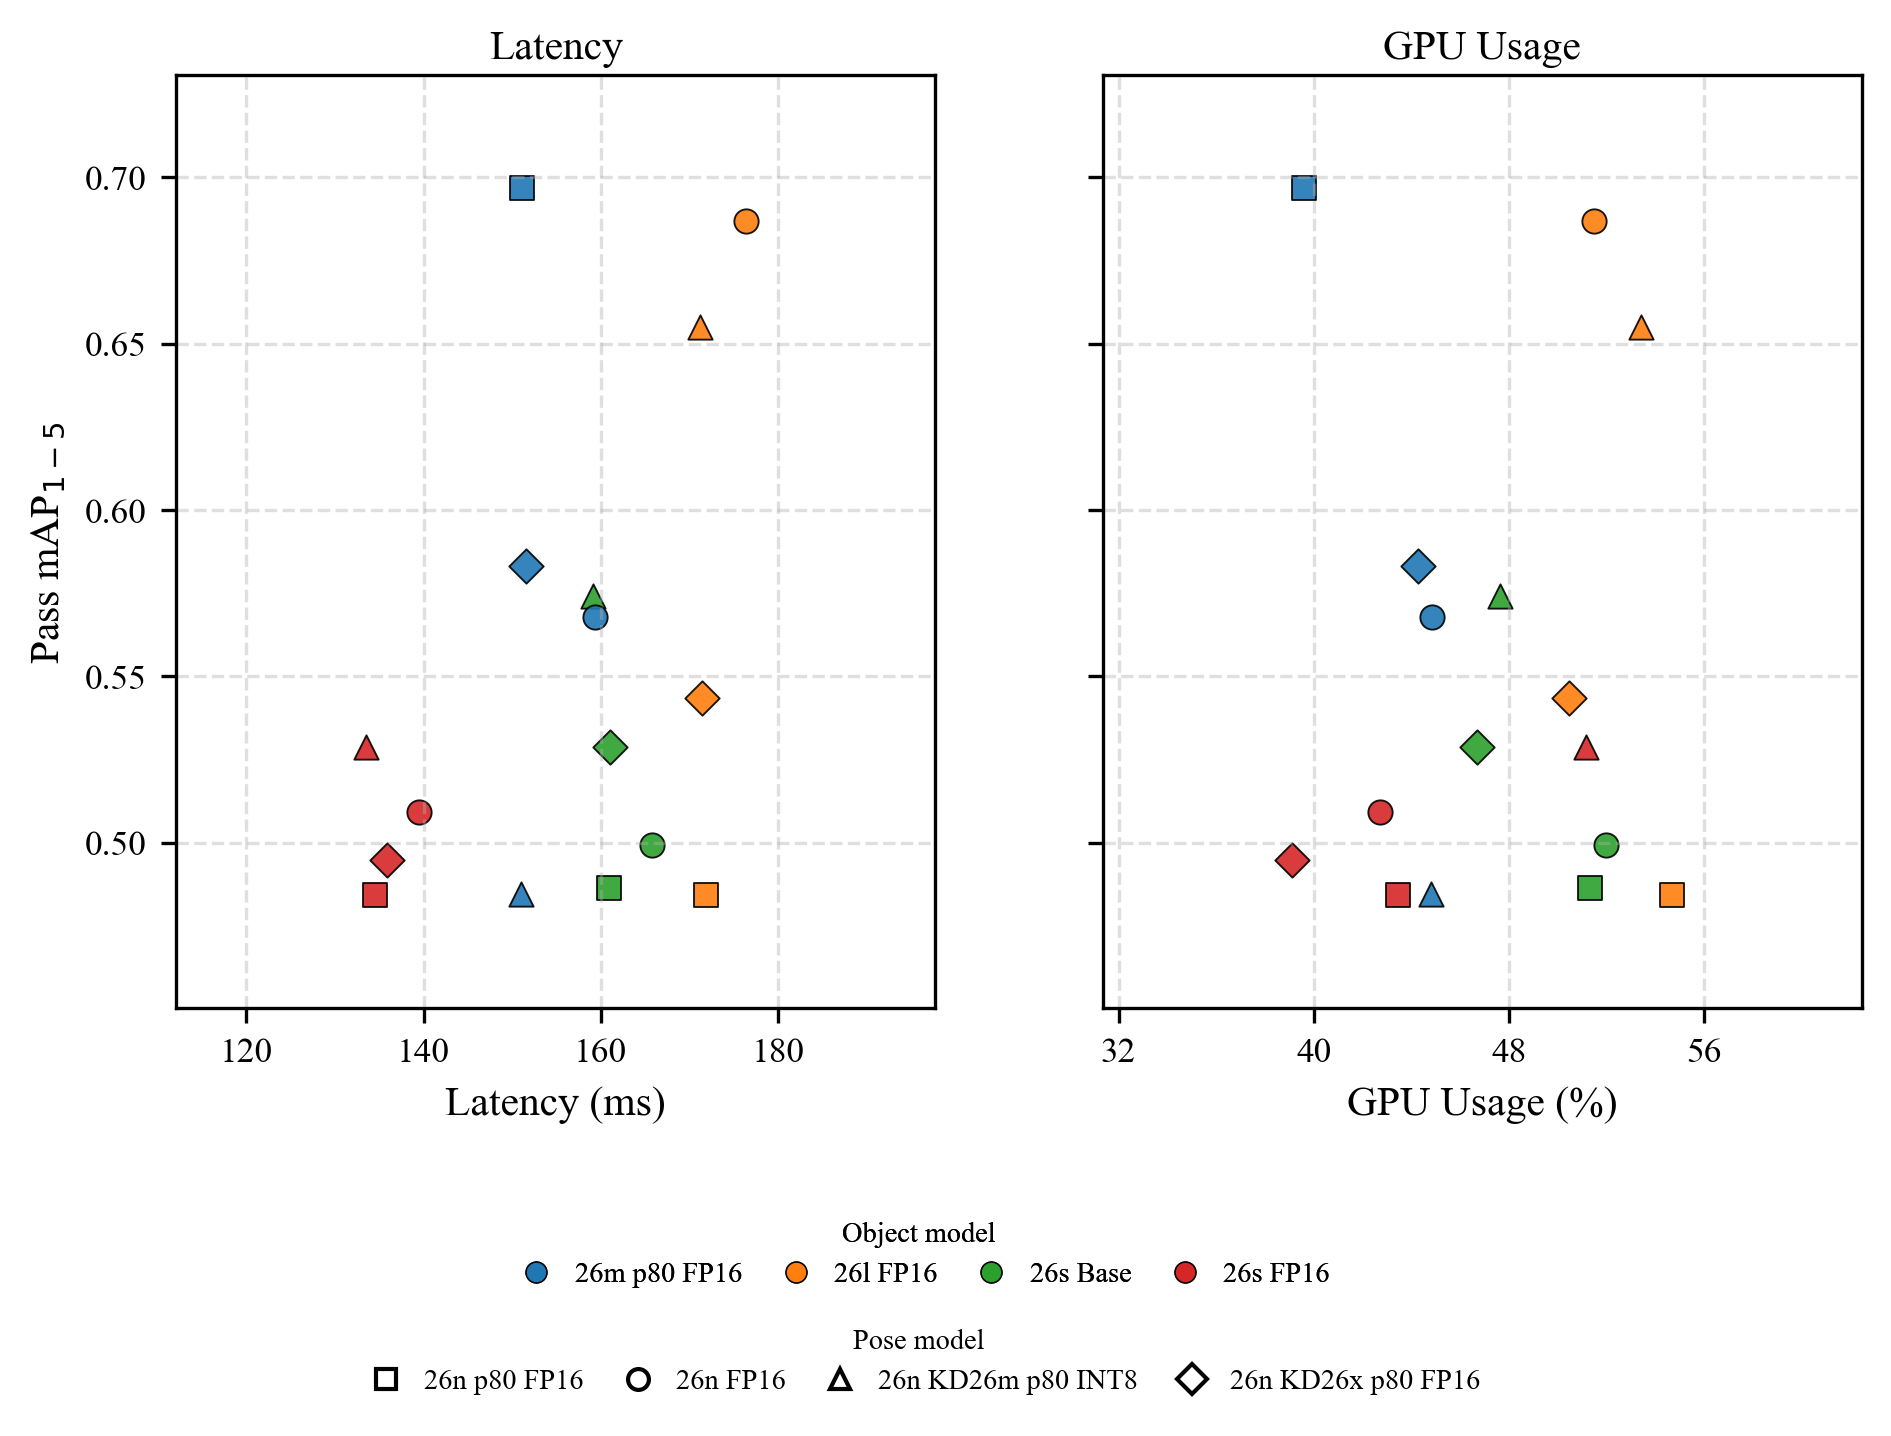
\includegraphics[width=\linewidth]{../Figures/produced_images/fullstack_rank02_map1_5_vs_latency_gpu_pair.png}
\end{figure}

\begin{figure}[H]
    \centering
    \caption{Pass mAP$_{1\text{--}5}$ versus thermal and power metrics for rank-02 full-stack combinations.}
    \label{fig:fullstack_rank02_thermal_tradeoffs}
    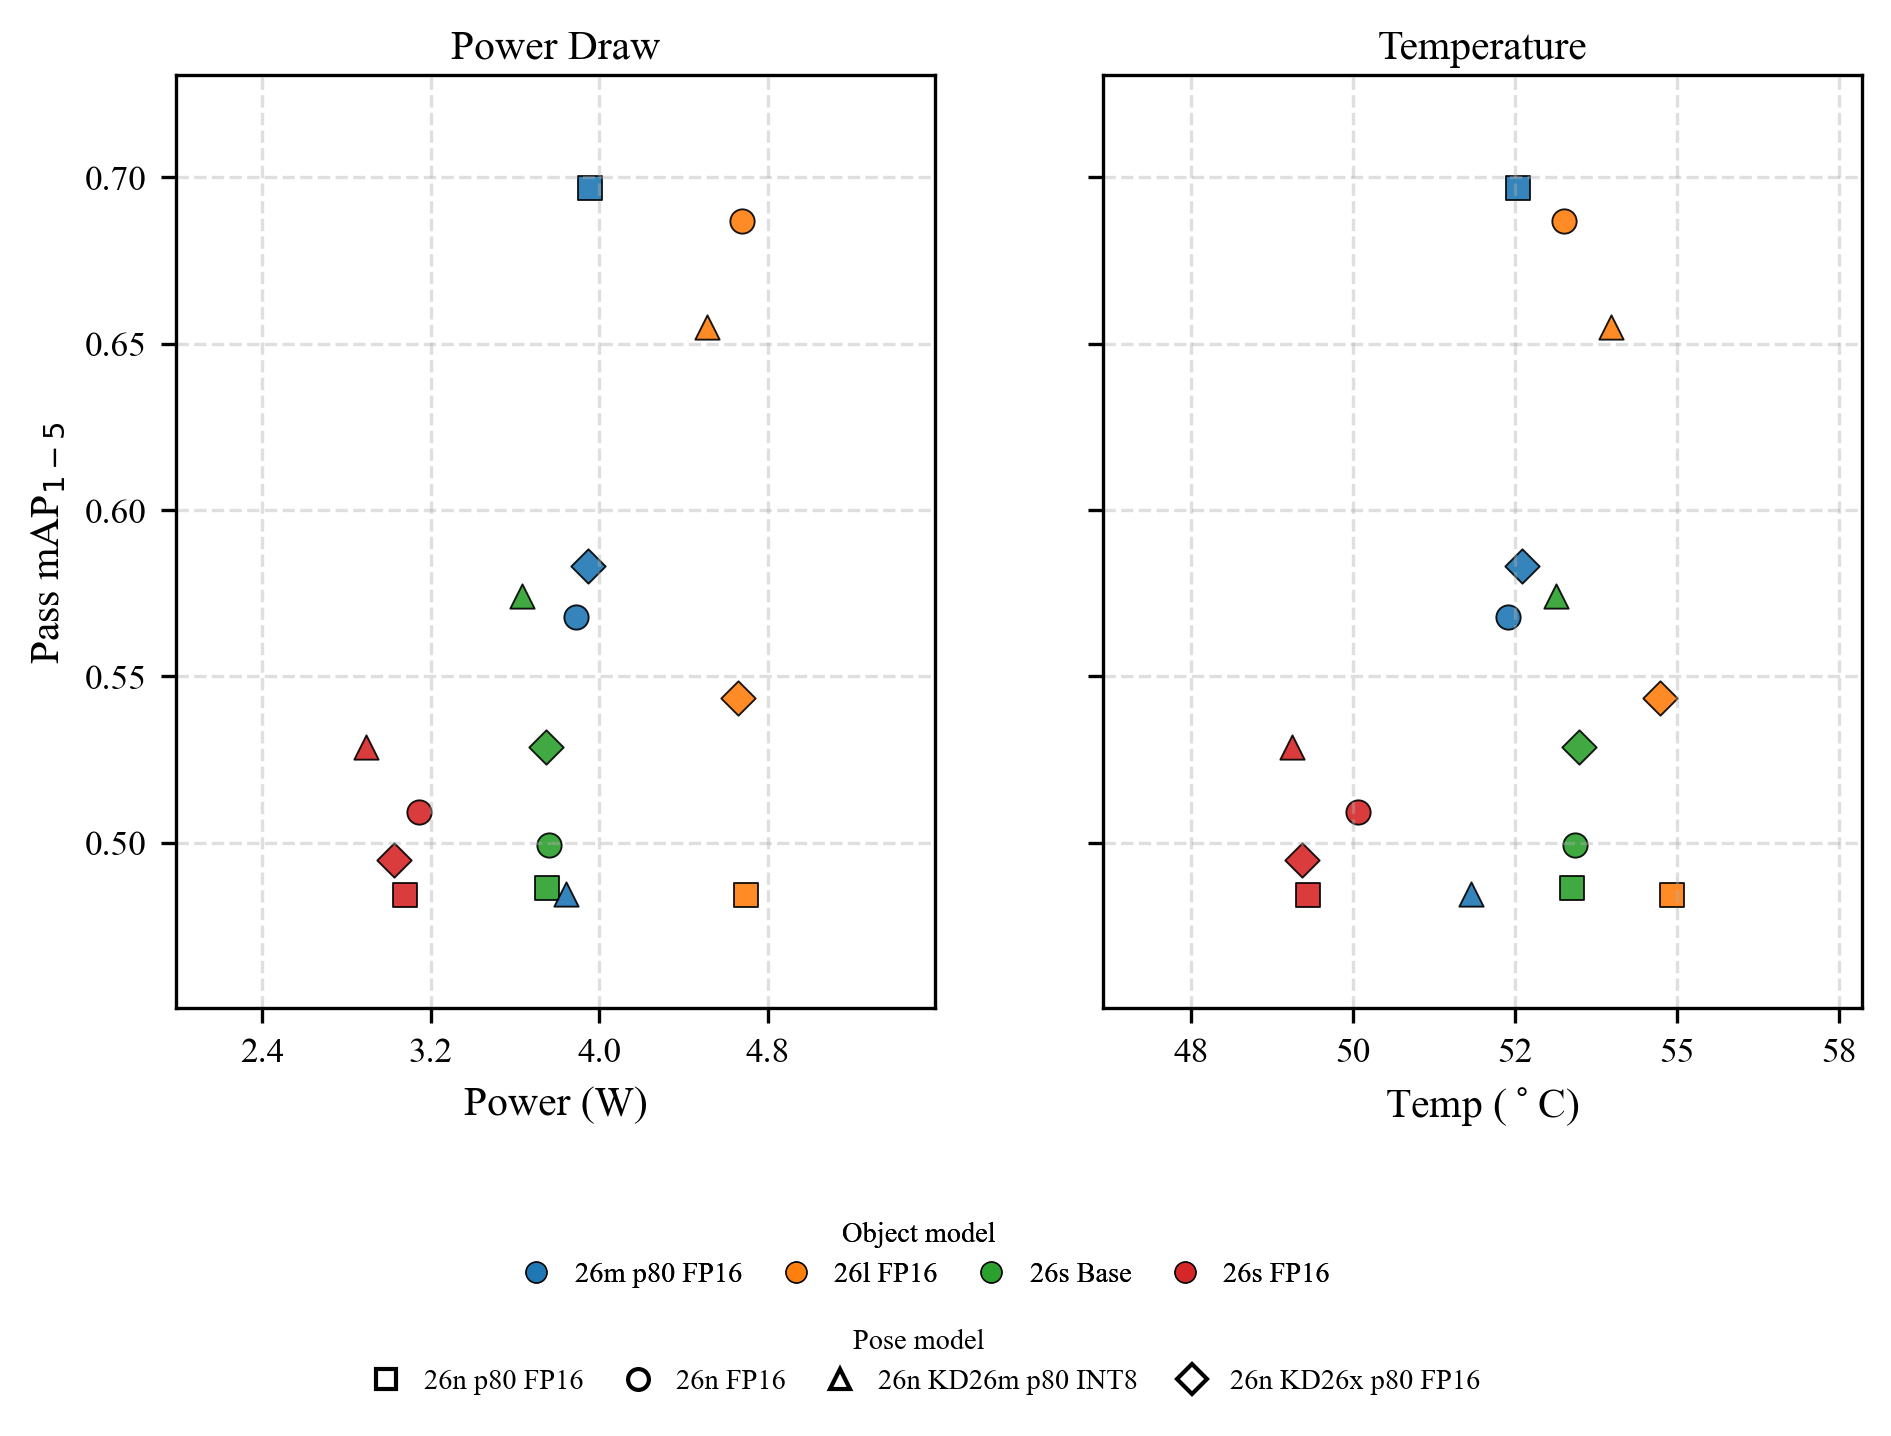
\includegraphics[width=\linewidth]{../Figures/produced_images/fullstack_rank02_map1_5_vs_power_temp_pair.png}
\end{figure}

Taken together, these figures show that the strongest pass-detection results do not require the highest hardware load within the tested full-stack shortlist. The higher-performing combinations cluster within a fairly narrow operating band, with only moderate variation in GPU usage, power draw, and temperature, while the latency plot shows that the best analytical scores are not confined to the slowest configurations. This reinforces the conclusion from Table~\ref{tab:fullstack_rank02_hardware_avg}: the system operates comfortably within the limits of the NVIDIA Jetson Orin Nano Dev Kit, with power draw far below the 25\,W budget, temperature well under the 85$^\circ$C limit, and GPU utilisation below 55\% in every case. The systems reached effective throughputs of roughly 11--13 FPS, near-real-time. Although this still falls short of strictly real-time (generally considered 20--25 FPS in broadcast video), the remaining gap is small, suggesting that full real-time deployment could likely be achieved through further system-level optimisation, rather than substantial additional model compression.

